\documentclass[11pt]{scrartcl}

\usepackage[utf8]{inputenc}
\usepackage[T1]{fontenc}
\usepackage{lmodern}
\usepackage[ngerman]{babel}
\usepackage{amsmath}
\usepackage{graphicx}
\usepackage{subcaption}
\usepackage{wrapfig}
\usepackage{float}
\usepackage[printonlyused, footnote]{acronym}
\usepackage[
    colorlinks=true,
    urlcolor=blue,
    linkcolor=black,
    citecolor=black
]{hyperref}
\usepackage[font={scriptsize},figurename=Bild]{caption}
\usepackage{listings}
\usepackage{color}

\definecolor{darkGreen}{rgb}{0,0.6,0}
\definecolor{gray}{rgb}{0.5,0.5,0.5}
\definecolor{mauve}{rgb}{0.58,0,0.82}
\definecolor{lightgray}{rgb}{.9,.9,.9}

\lstdefinelanguage{JavaScript}{
    keywords={typeof, new, true, false, catch, function, return, null, catch, switch, var, if, in, while, do, else, case, break, for},
    keywordstyle=\color{blue}\bfseries,
    ndkeywords={class, export, boolean, throw, implements, import, this},
    ndkeywordstyle=\color{darkGray}\bfseries,
    identifierstyle=\color{black},
    sensitive=false,
    comment=[l]{//},
    morecomment=[s]{/*}{*/},
    commentstyle=\color{darkGreen}\ttfamily,
    stringstyle=\color{mauve}\ttfamily,
    morestring=[b]',
    morestring=[b]"
}
\renewcommand*{\lstlistingname}{Code}

\lstset{frame=tb,
    language=JavaScript,
    backgroundcolor=\color{lightgray},
    extendedchars=true,
    basicstyle=\footnotesize\ttfamily,
    showstringspaces=false,
    showspaces=false,
    numbers=left,
    numberstyle=\footnotesize,
    numbersep=9pt,
    showtabs=false,
    captionpos=b
    aboveskip=3mm,
    belowskip=3mm,
    columns=flexible,
    breaklines=true,
    breakatwhitespace=true,
    tabsize=3
}

\title{MASTER THESIS}
\author{Oliver Becker}
\date{31. Oktober 2019} %%\today
\begin{document}

\par\vspace{-1cm}
\begin{flushright}
    \includegraphics[width=0.4\linewidth]{images/logo.png}
\end{flushright}
\vspace{1cm}\noindent
\begin{center}
    \huge MASTER THESIS\\
    \huge \color{red} Vorabversion 0.97\\
    \large Stand: \today
\end{center}
\vspace{1cm}\noindent
{\large Title:  Abgleich von LED Lichtquellen auf Basis einer komplexen Lichtsteuerung}
\par\vspace{3cm}\noindent
Submitted by: \hspace{2cm}             Oliver Becker\\
\\
Matriculation number:  \hspace{.6cm}   725810\\
\par\vspace{2cm}\noindent
1st Academic Supervisor: \hspace{.2cm} Prof. Dr. Herbert Krauß\\
\\
2nd Academic Supervisor: \hspace{.05cm} Prof. Dr. Shun-Ping Chen\\
\\
Industrial Supervisor:   \hspace{.75cm} Dipl.-Ing. Hartmut Cordes\\
\par\vspace{2cm}\noindent
Completion Date: \hspace{1.5cm}         31.10.2019
\clearpage

%%%%%%%%%%%%%%%%%%%%%%%%%% Template Content %%%%%%%%%%%%%%%%%%%%%%%%%%%%%%%%%%%%%%%%%%%%%%%%%%%%%%%%%%%%%%%
\noindent
Student:\\
\\
Oliver \hspace{6cm} Becker\\
\\
Date of Birth: 21.07.1992 \hspace{2.8cm} Matr-No.:725810
\par\noindent\rule{\textwidth}{0.4pt}
1st Academic Supervisor: Prof. Dr. Herbert Krauß\\
\\
2st Academic Supervisor: Prof. Dr. Shun-Ping Chen
\par\noindent\rule{\textwidth}{0.4pt}
Title: Abgleich von LED Lichtquellen auf Basis einer komplexen Lichtsteuerung\\
%%%%%%%%%%%%%%%%%%%%%%%%%% Abstract %%%%%%%%%%%%%%%%%%%%%%%%%%%%%%%%%%%%%%%%%%%%%%%%%%%%%%%%%%%%%%%%
\par\vspace{-0.8cm}\section*{Abstract}
\addcontentsline{toc}{section}{Abstract}
to be filled\\
to be filled\\
to be filled\\
to be filled\\
to be filled\\
to be filled\\
to be filled\\
to be filled\\
to be filled\\
to be filled\\
\par\noindent\rule{\textwidth}{0.4pt}
In partial fulfillment of the requirements of the University of Applied Sciences Hochschule
Darmstadt (h\_da) for the degree Master of Science in Electrical Engineering carried out in
collaboration with Industrial Enterprise\\
\\
Company:\hspace{0.45cm} MA Lighting Technology GmbH\\
Address:\hspace{0.7cm} Dachdeckerstraße 13\\
\hspace*{2.15cm} 97297 Waldbüttelbrunn\\
\\
This Master Thesis is subject to a non-disclosure agreement between the University of Applied 
Sciences Hochschule Darmstadt (h\_da) and the industrial partner.\\
\par\noindent\rule{\textwidth}{0.4pt}
(Signature)\\

1st Academic Supervisor:..............................................................................
\clearpage

%%%%%%%%%%%%%%%%%%%%%%%%%% Declaration %%%%%%%%%%%%%%%%%%%%%%%%%%%%%%%%%%%%%%%%%%%%%%%%%%%%%%%%%%%%%%%
\noindent
Student:\\
\\
Oliver \hspace{6cm} Becker\\
\\
1st Academic Supervisor: Prof. Dr. Herbert Krauß\\
\\
2st Academic Supervisor: Prof. Dr. Shun-Ping Chen
\section*{Declaration}
\addcontentsline{toc}{section}{Declaration}
I hereby declare that this thesis is a presentation of my original research work and that no other sources were used other
than what is cited.\\
I furthermore declare that wherever contributions of others are involved, this contribution is indicated, clearly
acknowledged and due reference is given to the author and source.\\
I also certify that all content without reference or citation contained in this thesis is original work.\\
I acknowledge that any misappropriation of the previous declarations can be considered a case of academic fraud.
\par\vspace{2cm}\noindent
Darmstadt, den 30.10.2019 \hspace*{0pt}\hfill Oliver Becker
\clearpage

%%%%%%%%%%%%%%%%%%%%%%%%%% tableofcontents %%%%%%%%%%%%%%%%%%%%%%%%%%%%%%%%%%%%%%%%%%%%%%%%%%%%%%%%%%%
\tableofcontents
\clearpage

%%%%%%%%%%%%%%%%%%%%%%%%%% Vorwort %%%%%%%%%%%%%%%%%%%%%%%%%%%%%%%%%%%%%%%%%%%%%%%%%%%%%%%%%%%%%%%%
\section*{Vorwort}
\addcontentsline{toc}{section}{Vorwort}
Weltweit finden große Veranstaltungen statt. Bei allen Inszenierungen spielt das Licht eine 
große Rolle. Egal, ob einfach nur hell oder szenisch ausgeleuchtet, bedarf es einer Steuerung 
für diese Lichttechnik. Bühnen und Ansprüche der Veranstalter werden immer größer und komplexer. 
So geht es über das einfache An- und Ausschalten eines Scheinwerfers schon sehr weit hinaus. 
Heutzutage werden Lichtanlagen mit leistungsfähigen Computersystemen gesteuert, welche von 
geschultem Personal bedient werden müssen.\\
In der Filmindustrie spielt Licht eine große Rolle. Die Ausleuchtung eines Film-Sets entscheidet 
auch wie die Handlung vom Betrachter wahrgenommen wird. Dies gilt sowohl für statische Szenen, 
als auch für die zumeist hoch aufwändigen dynamischen Installationen.
Eine der zurzeit größten Herausforderungen stellt die korrekte Farbwiedergabe der mannigfaltigen 
Lichtquellen an einem Film-Set dar.
Dies wird vor allem durch die unterschiedlichen chromatischen Eigenschaften von den Licht 
emittierenden Quellen erschwert. Diese Quellen sind heute überwiegend LEDs.\\
Als Beispiel wird hier ein Film-Set für eine Motorrad Verfolgungsszene genommen. Hier wird im 
Hintergrund mit großen LED Kacheln der computergenerierte Hintergrund abgespielt. Mit kleinen 
LED Streifen links und rechts neben dem im Studio aufgebauten Motorrad wird dynamisch Licht auf 
den Schauspieler emittiert, um eine größere Dynamik zu simulieren.
Zusätzlich wird mit kleinen Bildschirmen weiterer computergenerierter Hintergrund von vorne auf 
das Motorrad und den Schauspieler projiziert, um realistische Spiegelungen in der 
Windschutzscheibe und der Brille des Schauspielers zu erhalten.\\
Alle diese aufgezählten Emitter haben zumeist alle unterschiedlichste chromatische Kennwerte 
sofern diese überhaupt bekannt sind. Ein Abgleich dieser Quellen ist wünschenswert für ein 
homogeneres Farbbild.
\clearpage

%%%%%%%%%%%%%%%%%%%%%%%%%% MA Lighting Technology %%%%%%%%%%%%%%%%%%%%%%%%%%%%%%%%%%%%%%%%%%%%%%%%%%
\section{MA Lighting Technology}
MA Lighting Technology GmbH (im Folgenden MA) wurde 1983 von Michael Adenau zusammen mit
den drei Mitgesellschaftern Ernst Ebrecht, Thomas Stanger und Werner Hauptvogel gegründet. MA
entwickelt und produziert Lichtsteuerungen für die Bereiche Fernsehen, Veranstaltungen, Theater
und szenische Gebäudebeleuchtung. Schon Anfang der 1990er Jahre erkannten die Firmengründer
das Potenzial der elektrischen und digitalen Steuerung von Scheinwerfern und bauten die ersten
Lichtstellpulte, sowie die zugehörigen Komponenten. Im Laufe der Jahre entwickelte sich MA zu
einem der international führenden Unternehmen für computergesteuerte Lichtstellpulte,
Netzwerkkomponenten und digitale Dimmer Systeme.\\
In der Referenzliste von MA findet man viele große internationale Theater und Opernhäuser, Bands
von AC/DC über Sting bis U2, die Eröffnungsfeier der Olympischen Spiele, den Eurovision Song
Contest 2019 oder die Lichtinstallation zum 25. Jahrestag des Falls der Berliner Mauer 2014.\\
\begin{wrapfigure}{r}{0.5\textwidth}
    \vspace{-25pt}
    \begin{center}
        \includegraphics[width=0.48\textwidth]{images/csm_MA_building_WBB.jpg}
    \end{center}
    \vspace{-20pt}
    \caption{Firmensitz Waldbüttelbrunn}
    \vspace{-15pt}
\end{wrapfigure}
Der Hauptsitz der MA Lighting Technology GmbH befindet sich in Waldbüttelbrunn in der Nähe von
Würzburg. Dort beschäftigt MA circa 100 Mitarbeiter. In den fünf Gebäuden befinden Soft- und
Hardwareentwicklung, Testabteilung, Produktion, Lager und Management. Alle Produkte werden
größtenteils von Hand von den Mitarbeitern vor Ort zusammengebaut. Platinen und Gehäuse werden
von externen Firmen geliefert. Die einzelnen Bauteile werden von den Mitarbeitern auf den
Platinen aufgesteckt und verlötet. Anschließend werden die bestückten Platinen in den Gehäusen
montiert und verkabelt. Nach einem mehrtägigen BurnIn-Test und einer Werkskonfiguration werden
die Geräte verpackt und sind versandfertig.\\
\\
Kundensupport und Vertrieb werden in Deutschland von der externen Firma MA Lighting International
durchgeführt. Diese hat ihren Sitz in Paderborn. Die Konsultation der Mitarbeiter in
Waldbüttelbrunn erfolgt lediglich bei größeren technischen Fragen und Problemen.\\
Eines der ersten Produkte von MA war der Lightcommander24, eine analoge Lichtsteuerkonsole auf
Basis des \ac{dmx} Protokolls von 1990. Nach kurzer Zeit folgten Dimmer für
Scheinwerfer und \ac{dmx}-Demultiplexer, um analoge Geräte ansteuern zu können.\\
\begin{figure}[H]
    \centering
    \begin{subfigure}[b]{0.45\textwidth}
        \includegraphics[width=\textwidth]{images/grandMA_1.png}
        \caption{grandMA ful-Size}
    \end{subfigure}
    \hfill 
    \begin{subfigure}[b]{0.25\textwidth}
        \includegraphics[width=\textwidth]{images/MA_2Port_Node_onPC_13019x.png}
        \caption{2Port Node}
    \end{subfigure}
    \caption{grandMA 1 Serie Produkte}\label{fig:gma1}
\end{figure}
\noindent
Ebenso entwickelte MA die Steuerpulte Scan-Commander und die grandMA Series 1 sowohl als
Konsole, als auch als Computerapplikation. Das Besondere an dieser Technologie ist, dass \ac{dmx}-Daten
nicht nur über \ac{xlr}, sondern auch über ein eigenes Ethernet-Netzwerkprotokoll namens 'MA-Net'
ausgegeben werden. Als Gegenstück am anderen Ende des Netzwerkkabels existieren sogenannte
\ac{dmx}-Nodes. Diese fungieren als Protokollwandler zwischen MA-Net und \ac{dmx}.\\
Die Firma setzte immer wieder Standards in der Branche. Im Zuge des technischen Fortschritts –
Einsatz von \ac{led}s als Lichtquelle, moderne Netzwerktechnologie und Videodatenverarbeitung –
wurde die Produktpalette wesentlich erweitert. Hinzu kam die grandMA2 Series.\\
\begin{figure}[H]
    \centering
    \begin{subfigure}[b]{0.45\textwidth}
        \includegraphics[width=\textwidth]{images/MA_grandMA2_full-size.png}
        \caption{grandMA2 full-size}
    \end{subfigure}
    \hfill 
    \begin{subfigure}[b]{0.4\textwidth}
        \includegraphics[width=\textwidth]{images/MA-VPU-plus_d.png}
        \caption{VPU}
    \end{subfigure}
    \caption{grandMA 2 Serie Produkte}\label{fig:gma2}
\end{figure}
\noindent
Die grandMA2 Series ist die moderne Fortführung der grandMA Series 1. Außerdem stellt sie
folgende Produkte bereit: Die Network Processing Unit (NPU), eine Prozessoreinheit, welche die
Konsole in ihren Berechnungen unterstützt, indem die Konsole Rechenaufträge auf die NPU dezentral
auslagert. Die Video Processing Unit (VPU) verarbeitet Video-Content und gibt diesen nativ über
Grafikkarten oder Pixelmapping mit Hilfe von \ac{dmx} aus. Die Replay-Unit (RPU) ist eine vollwertige
Konsole ohne die typischen Steuerelemente, sie dient beispielsweise als Havariegerät. Zuletzt noch
verschiedene Variationen der Nodes, welche weiterhin als Protokollwandler dienen.\\
Alle diese Produkte adressieren vor allem den Highend-Profibereich für Theaterproduktionen,
Liveshows und Festinstallationen.\\
\begin{figure}[H]
    \includegraphics[width=\textwidth]{images/grandMA3-full-size.png}
    \caption{grandMA3 full-size}\label{fig:gma3}
\end{figure}
\noindent
Seit Mitte 2017 entwickelt MA eine neue Produkt Serie. Die grandMA3 Serie. Diese Serie greift die
in den letzten 34 Jahren gesammelte Erfahrung auf, jedoch wurde jede Zeile Code neu geschrieben,
um die technischen Möglichkeiten der neuen Hardware vollumfänglich nutzen zu können.\\
Neben vielen Veränderungen gegenüber den Vorserien arbeitet die Farblogik der grandMA3 Software
mit den Spezifikationen des \ac{cie} 1931 Standards.
\clearpage

%%%%%%%%%%%%%%%%%%%%%%%%%% Grundlagen %%%%%%%%%%%%%%%%%%%%%%%%%%%%%%%%%%%%%%%%%%%%%%%%%%%%%%%%%%%%%%%%%%%%
\section{Grundlagen}
In dieser Arbeit werden Lichtquellen mit der grandMA3 Applikation von MA Lighting über ein Protokoll
mit der Bezeichnung \ac{dmx} angesteuert.\\
Für eine erste Überprüfung geeigneter Hardware wurde mit einer kleinen Demo Applikation gearbeitet. Diese wurde
in JavaScript und \ac{html} mit Hilfe des Electron Frameworks erstellt.\\
Weiter wird diese Applikation für die Ausgabe von \ac{dmx} genutzt.\\
Im Folgenden werden die hier verwendeten Protokolle, Programme, und Frameworks dargelegt.

\subsection{DMX}
Diese Abkürzung steht für Digital Multiplex. Dahinter verbirgt sich ein digitales Steuerprotokoll,
welches vornehmlich in der Veranstaltungstechnik eingesetzt wird. Es wurde zuerst als DMX-
512/1990 standardisiert. Im November 2004 wurde dieser Standard aktualisiert, bekannt als
DMX512-A (ANSI E1.11-2008). \ac{dmx} basiert elektrisch auf dem seriellen RS-485 (EIA-485)
Schnittstellenstandard.\\
\begin{figure}[H]
    \includegraphics[width=\textwidth]{images/dmx.png}
    \caption{Physikalische Übertragung DMX-512/1990 (RS-485)}
\end{figure}
\noindent
Das eigentliche Signal wird dabei seriell auf einem Leitungspaar symmetrisch übertragen - auf der
einen Leitung mit invertierten und auf der anderen mit nichtinvertiertem Pegel. Das Signal ist so
weniger störungsempfindlich, da sich externe Einstreuungen auf beide Datenleitungen gleichmäßig
auswirken und am Empfänger nicht das Pegelniveau, sondern die Pegeldifferenz ausgewertet wird.
Das ermöglicht laut Standard [2] bis zu 1200m lange Übertragungsstrecken und eine
Datenübertragungsrate bis zu 12 \ac{MBps}. Ein Netzwerk aus mehreren Geräten wird als Bus aufgebaut.\\
Die Datenübertragung erfolgt mittels einer \ac{uart} gesteuerten asynchronen seriellen Schnittstelle. Ein
Datenframe besteht aus acht Datenbits und zwei Stoppbits. Die Symbolrate beträgt 250 kBaud (Baud = Bits pro sec).
\begin{figure}[H]
    \includegraphics[width=\textwidth]{images/DMX_zeitlich.png}
    \caption{Zeitliche Darstellung \ac{dmx}-Signal}
\end{figure}
\noindent
\begin{table}[H]
    \small
    Legende zu Bild 6:\\
    \begin{tabular*}{\textwidth}{l @{\extracolsep{\fill}} llllll}
        Nr. & Signalabschnitt & Min & Soll & Max & Einheit\\
        1 & BREAK & 88 & 176 & - & $\mu$s\\
        2 & MARK after BREAK & 8 $\mu$s & - & < 1 s\\
        3 & Slot Time & 43,12 & 44,0 & 44,88 & $\mu$s\\
        4 & Startbit & 3,92 & 4,0 & 4,08 & $\mu$s\\
        5 & LSB (niederwertigstes Datenbit) & 3,92 & 4,0 & 4,08 & $\mu$s\\
        6 & MSB (höchstwertiges Datenbit) & 3,92 & 4,0 & 4,08 & $\mu$s\\
        7 & Stoppbit & 3,92 & 4,0 & 4,08 & $\mu$s\\
        8 & MARK Inter-Slot Time & 0 & - & < 1 & s\\
        9 & MARK before BREAK & 0 & - & < 1 & s\\
        10 & BREAK – BREAK (Übertragungsausfall) & 1,2 ms & - & 1,25 s & s\\
    \end{tabular*}
\end{table}
\noindent
Ein \ac{dmx}-Paket beginnt mit mindestens 88 $\mu$s (22 Bitlängen) niedrigem Pegel (logisch 0) – dieser
Abschnitt wird 'BREAK' genannt. Durch ihn wird eine einfache Erkennung des Paketanfangs
ermöglicht, da quasi jeder handelsübliche UART den Break als ungültiges Datenbyte mit fehlenden
Stoppbits meldet. Darauf folgt 'MARK after BREAK' mit mindestens 8 $\mu$s (2 Bitlängen) hohem Pegel /
Ruhezustand des Daten-Busses (logisch 1). In dieser 'MARK'-Zeit können sich langsamer getaktete
Controller auf ein neues \ac{dmx}-Paket einstellen. Dann wird das Startbyte mit dem Wert 0 für \ac{dmx}
übertragen. Das Startbyte ist der Slot 0. Anschließend werden die anderen 512 Slots mit den
relevanten \ac{dmx}-Daten gesendet. Es können, müssen aber nicht alle 513 Slots übertragen werden.
Eine Adressierung der Slots ist jedoch nicht möglich – der zweite gesendete Slot ist für den ersten
Kanal, der dritte Slot für den zweiten Kanal etc.. Sollte die Übertragung zu einem beliebigen
Zeitpunkt unterbrochen werden, kann sie durch das Senden eines neuen \ac{dmx}-Paketes wieder
aufgenommen werden. Die 'BREAK'-Sequenz führt automatisch zu einem Zurücksetzen aller noch
offenen Übertragungen.\\
In der Spezifikation DMX512-A wurden erstmals Maximalzeiten für die Slot Time (3) und den
zeitlichen Abstand zwischen zwei BREAKs (10) definiert. Wenn die Zeit zwischen zwei BREAKs größer
als eine Sekunde ist, wertet ein Empfänger dies als Übertragungsausfall. Ein Übertragungsausfall ist
folgendermaßen definiert: 'Ein Übertragungsausfall kann dann angenommen werden, wenn der
angeschlossene Empfänger nicht innerhalb der angegebenen Zeit einen gültigen BREAK mit
darauffolgendem NULL-Startcode erkennen kann.' Weiter wurde eine empfohlene Länge des
BREAKs definiert. Dies soll den Empfängern die Dekodierung erleichtern.
\clearpage

\subsection{Art-Net}
Art-Net ist ein Netzwerkprotokoll, dass zur Verteilung von \ac{dmx} und \ac{rdm} Daten genutzt werden kann.
Es ist in OSI Layer 4 auf UDP aufgebaut. Das Protokoll ist von der Firma Artistic Licence Holdings Ltd. lizenziert.\\
In dieser Arbeit wird Art-Net in der dritten Version verwendet. Diese Version wurde 2011 publiziert.\\
Über das Art-Net 3 Protokoll können bis zu 32.768 \ac{dmx} Universen verwaltet werden.\\
\cite{artnet}\\
Das Protokoll kann sowohl Unicast, Multicast oder Broadcast eingesetzt werden. Somit können auch komplexe Netzwerke
in einer physikalischen Struktur aufgebaut werden.\\
\\
Mit Hilfe von Protokollwandlern wie dem MA xPort Node kann Art-Net in \ac{dmx} umgewandelt werden. Auch von anderen
Herstellern gibt es auf dem Markt weit verbreitete Protokollwandler.\\
\\
Art-Net IP Adressen sind nach folgendem Muster aufgebaut:
\begin{table}[H]
    \begin{tabular*}{\textwidth}{l @{\extracolsep{\fill}} lllll}
        Bytes & 4 & 3 & 2 & 1\\
        IP Adresse & Netz & Netz & Host & Host\\
        Subnetz & 255 & 255 & 0 & 0\\
    \end{tabular*}
\end{table}
\noindent
In der Regel werden IP Adressen für Art-Net mit dem Netz 2.X.X.X oder 10.X.X.X verwendet. Art-Net wird über den
Netzwerkport 6454 gesendet und empfangen.\\
Ein Art-Net Paket kann verschiedene Informationen enthalten. Hier sendet die Applikation jedoch
lediglich ArtDmx Pakete. Diese Pakete transportieren DMX Daten. Hier ist der Aufbau des ArtDmx Paketes dargelegt.\\
\begin{table}[H]
    \begin{tabular*}{\textwidth}{l @{\extracolsep{\fill}} lll}
        Byte Offset & Name & Größe & Beschreibung\\
        0 & ID & 8 & Art-Net\\
        8 & OpCodeLo & 1 & Pakettyp (ArtDmx) LSB\\
        9 & OpCodeHi & 1 & Pakettyp (ArtDmx) MSB\\
        10 & ProtVer & 2 & Protokollversion (14)\\
        12 & Sequenz & 1 & Paketsequenznummer\\
        13 & Physical & 1 & Physikalischer Port\\
        14 & Universe & 2 & Art-Net Universum\\
        16 & Length & 2 & Länge der DMX Daten\\
        18 & Data[] & 2-512 & DMX Daten\\
    \end{tabular*}
    \caption{Aufbau des ArtDmx Pakets}\label{tab:ArtDmxDefinition}
\end{table}
\noindent
\cite{artdmx}
\clearpage

\subsection{HTML, JavaScript, CSS}
\ac{html} ist eine Strukturbeschreibungssprache. Sie ist an den \ac{xml} Standard angelehnt. \ac{html}
wird hauptsächlich in der Webentwicklung verwendet. Doch kann \ac{html} auch für webgestützte Desktop
Applikationen genutzt werden.\\
Die Sprache enthält grundlegende Elemente zur Beschreibung von Tabellen, Einbindung von Medieninhalten sowie
von weiteren HTML Dateien.\\
Allerdings ist das erzeugte Ergebnis (zum Beispiel von einem Webbrowser) meist statisch. Als Beispiel ändert sich
der Inhalt nicht mit dem Vergrößern oder Verkleinern des Webbrowsers für eine bessere Lesbarkeit. Um solche heute
gewohnten Effekte zu erzeugen, benötigt man \ac{css} oder JavaScript.\\
\\
\ac{css} ist eine in der \ac{json} Notation geschriebene Sprache. Hier kann auf Elemente in einem \ac{html} Baum
verwiesen werden, und mit verschiedenen Attributen das Erscheinungsbild im Webbrowser oder in der Applikation
geändert werden.\\
Einfache Dinge wie Hintergrund- oder Textfarben bis hin zu komplexen Animationen können mit \ac{css} beschrieben
werden.\\
\\
JavaScript ist eine Skript Sprache, die wie \ac{css} meist in der Webentwicklung verwendet wird, kann jedoch
mit einer entsprechenden JavaScript Laufzeitumgebung auch ohne Browser auf Endgeräten ausgeführt werden.\\
Bei dieser Arbeit muss zwischen zwei Arten der Nutzung der Sprache JavaScript unterschieden werden:\\
\begin{addmargin}[2em]{0em}
 - Webcode, welcher innerhalb des Webbrowsers augeführt wird.\\
 - Appcode, welcher mit der NodeJS Laufzeitumgebung auf dem Endgerät ausgeführt wird.\\
\end{addmargin}
NodeJS ist eine JavaScript Laufzeitumgebung. Laufzeitumgebungen sind zum Ausführen eines Programms in einer
Sprache zwingend erforderlich.\\
Webcode kann dynamisch auf einer Website durch anklicken eines \ac{html} Elements weitere HTML Elemente erzeugen,
oder existierende manipulieren oder löschen. Somit kann eine Benutzereingabe das gesamte Erscheinungsbild ändern,
ohne eine andere \ac{html} Seite aufzurufen.
Zusätzlich bieten Webbrowser sogenannte "'Storages"' oder Speicher. Dort können mit JavaScript Daten gespeichert werden,
um diese zum Beispiel beim nächsten Aufruf dieser Seite weiter zu nutzen.\\
Appcode hat gegenüber Webcode weitreichendere Befugnisse auf dem Endgerät wie Dateisystemzugriff und Zugriff auf
externe Schnittstellen, wie USB oder herkömmliche serielle Schnittstellen (COM).
\clearpage

\subsection{Electron}
Electron ist ein Framework, welches zum Erstellen von Desktop Anwendungen genutzt werden kann. Electron funktioniert
wie ein Webbrowser. Die Applikation zeigt \ac{html} und andere Textinhalte an.\cite{electron} Der Programmierer kann diese
Browserumgebung nach Belieben modifizieren und erweitern. Electron wurde aus dem Projekt Atom Editor von Github entwickelt.\\
Das Framework basiert auf dem Chromium Projekt von Google. Auf dem Chromium Projekt basiert auch der Chrome Webbrowser von
Google.\\
Das Electron Framework bietet eine betriebssystemübergreifende Applikation als Resultat. Electron Applikationen können unter
Windows, Linux und MacOS ausgeführt werden.\\
Electron ist Open Source Software und wird von einer breiten Community weltweit permanent weiterentwickelt.\cite{electron} Das Projekt wird
in den Programmiersprachen C++ und JavaScript geschrieben. Der JavaScript-Anteil wird mit NodeJS auf den Zielcomputern ausgeführt.\\
Electron selbst wird als Paket angeboten. Dies ist üblich für Open Source NodeJS Projekte. Ein Paket kann in ein Projekt eingebunden werden,
vergleichbar mit einem SDK und einer DLL für C++. In der Regel werden diese Pakete über den Netzwerk-Paket-Manager oder auch \ac{npm} von
Servern abgerufen. Weiter managed \ac{npm} die installierten Pakete pro Projekt, wie Versionen jedes Paketes, sowie das aktualisieren.

\subsection{Git und Github}
Git ist eine Datei Versionierungs- und Management Software. Git wird häufig in der Software Entwicklung mit mehreren Stationen eingesetzt.\\
Eine Instanz von einem mit Git verwalteten Dateisystem wird als Repository bezeichnet. Diese Instanz wird meist auf einem Server bereitgestellt.
Ein Nutzer kann den Inhalt des Repositories auf sein Endgerät abrufen.
Abgerufene Dateien, vornehmlich nicht binäre Textdateien, können anschließend lokal auf einem Endgerät editiert werden. Wenn eine neue Version
der Datei in das Repository eingestellt werden soll, werden die Änderungen an den Dateien mit einem Kommentar eingestellt (committed).
Diese eingestellten Änderungen werden dann mit dem Server synchronisiert und mit den Änderungen von anderen Stationen automatisch zusammengeführt.\\
\\
Dieses System macht das Entwickeln einer Software mit mehreren Entwicklern deutlich einfacher.\\
\\
Github ist eine Webplattform, welche kostenlos öffentliche Repositories hosted. Dort wurde auch das Git Repository der Applikation
dieses Projektes gehostet.\\
Zusätzlich bietet Github ein Projektverwaltungssystem.
\clearpage

%%%%%%%%%%%%%%%%%%%%%%%%%% Licht und Licht messen %%%%%%%%%%%%%%%%%%%%%%%%%%%%%%%%%%%%%%%%%%%%%%%%%%%%%%%%%%%%%%%
\section{Licht und Licht messen} \label{light and measurement}
Der Begriff Licht bezeichnet den Teil des elektromagnetischen Spektrums, welcher mit dem menschlichen Auge zu erfassen ist.\\
\\
Licht besteht aus rein physischer Betrachtungsweise aus Wellen im elektromagnetischen Spektrum und Teilchen. Dieses Phänomen, dass sich
Licht sowohl in der Ausbreitung wie eine Welle, als auch gleichzeitig ein wie Teilchen verhält, nennt sich Welle-Teilchen-Dualismus.
Dieser Begriff wurde durch Albert Einstein und Max Planck begründet. In dieser Theorie wird Licht als Quantenobjekt
beschrieben. \cite{wikiLicht}\\
\begin{wrapfigure}{r}{0.5\textwidth}
    \vspace{-25pt}
    \begin{center}
        \includegraphics[width=0.48\textwidth]{images/Elektromagnetisches-Spektrum.png}
    \end{center}
    \vspace{-20pt}
    \caption{Licht im elektromagnetischen Spektrum \cite{spectrumLight}}
    \vspace{-15pt}
\end{wrapfigure}
\noindent
Licht ist im elektromagnetischen Spektrum messbar. Somit kann man einen Farbton als eine Frequenz und eine Helligkeit als eine Amplitude beschreiben.
Wo eine Farbe im elektromagnetischen Spektrum einzuordnen ist, wird sie mit der Wellenlänge in Nanometern (nm) angegeben. Diese Zahl fällt von
dem Infrarotbereich des Spektrums ab 760 nm bis in den Ultraviolettbereich bei 380 nm.
\begin{align}\label{Equ:1}
    \lambda = \frac{c}{f}
\end{align}
Die zugehörigen Frequenzen liegen mit (\ref{Equ:1}) bei etwa 394,5 \ac{thz} für Infrarot und circa 789 \ac{thz} für Ultraviolett. Das
entspricht einer Bandbreite von 394,5 \ac{thz}, die das menschliche Auge erfassen kann.\\
\\
Dieser Teil des elektromagnetischen Spektrums lässt sich zum Beispiel mit Photodioden messen. Sensoren, welche eine solche Aufgabe erfüllen,
werden allgemein als Spektralsensoren bezeichnet.
\clearpage

%%%%%%%%%%%%%%%%%%%%%%%%%% Farbe %%%%%%%%%%%%%%%%%%%%%%%%%%%%%%%%%%%%%%%%%%%%%%%%%%%%%%%%%%%%%%%%%%%%%%
\section{Farbe}
Der Begriff Farbe, als Sinneseindruck, beschreibt die verschiedenen Zustände, welche die Amplituden im elektromagnetischen Spektrum annehmen können. Hier ist es
unerheblich, ob nur eine einzelne Spektrallinie oder eine breite spektrale Verteilung betrachtet wird.\\
Der Farbeindruck wird vorallem durch den Farbton geprägt. Ein Farbton entsteht natürlich oder künstlich von einem emittierenden oder reflektieren Körper.
Weiter ist die Sättigung ein entscheidendes Merkmal einer Farbe. Umso intensiver ein Farbton ist, desto höher ist die Sättigung der Farbe. Ein blasser
Farbton beinhaltet in seinem Spektrum einen Weiß-Anteil. Je blasser der Farbton, desto mehr Weiß-Anteile enthält er. Zuletzt ist noch die Helligkeit zu
nennen. Sie drückt die Intensität der Lichtempfindung einer Farbe aus und ist mit der Farbempfindung fest verknüpft.
\subsection{Farbtemperatur}
Der Begriff der Farbtemperatur ist durch den planckscher Strahler begründet. Es wurde beobachtet, dass sich beim starken Erhitzen eines Metalls
die Farbe des Metalls verändert. Ab einer Temperatur von etwa 923 Kelvin (K), also 650 Grad Celsius, fängt das Metall an rot zu glühen. Bei
weiterem Erhöhen der Temperatur wechselt der Farbton des Metalls über gelb zur sogenannten Weißglut ab rund 1300 Celsius (1573 K). % Weißglut ist kein neutral weiß 
\begin{figure}[H]
    \begin{center}
        \includegraphics[width=.8\textwidth]{images/thermal_radiation_figure.png}
    \end{center}
    \caption{Farbtemperatur Darstellung mit Kelvin Skala \cite{wikiFarbtemperatur}}
\end{figure}
\noindent
Dieses Prinzip der Lichtemittierung wird auch Temperaturstrahlung genannt.\\
Mit diesem Maß wird auch heute bei \ac{led}s noch die Farbtemperatur bestimmt und in Kelvin angegeben, auch wenn die Lichtemittierung nicht auf der
Temperaturstrahlung basiert.
\subsection{Farbmischung}
Die Farbmischung folgt zwei Prinzipien, welche im Folgenden dargelegt werden.
\subsubsection{Additiv}
Nimmt man eine rote und eine grüne Lichtquelle und lässt diese auf eine weiße, also neutrale, Fläche strahlen entsteht für das menschliche Auge
ein Sinneseindruck einer gelben Farbe. Dies geschieht spektral betrachtet durch eine Addition der Amplituden der einzelnen Wellenlängen.
\cite[62]{lichtquellen}\\
\begin{wrapfigure}{r}{0.5\textwidth}
    \vspace{-25pt}
    \begin{center}
        \includegraphics[width=0.48\textwidth]{images/additive_color_mixing.png}
    \end{center}
    \vspace{-20pt}
    \caption{Prinzip additive Farbmischung}
    \vspace{-15pt}
\end{wrapfigure}
Emittiertes Licht unterliegt generell der additiven Farbmischung. Dieses Prinzip findet beispielsweise Anwendung bei der Farbmischung von \ac{led}s.
Mit diesem Prinzip funktionieren alltägliche Gegenstände wie Bildschirme in Fernsehgeräten oder Smartphones.
\subsubsection{Subtraktiv}
Reflektiertes Licht unterliegt generell der subtraktiven Farbmischung. Nimmt man eine weiße Lichtquelle, enthält diese ein breites Spektrum an Wellenlängen.
Trifft das weiße Licht auf einen Körper, wird das Licht reflektiert. Jedoch können Körper einzelne Wellenlängen oder auch größere Wellenlängenbereiche
absorbieren. Absorbiert ein Körper vereinfacht rotes und blaues Licht und wird er von einer weißen Lichtquelle angestrahlt reflektiert er grünes
Licht. Dieses reflektierte Licht trifft nun das menschliche Auge. Somit erscheint der Körper grün.
\cite[62]{lichtquellen}\\
Besonders die subtraktive Farbmischung ist uns allgegenwärtig. Mit der Sonne oder der Raumbeleuchtung als weiße Lichtquelle sehen wir unsere Umgebung in
verschiedensten Farben und passen unsere Umgebung nach diesem Prinzip an. Von der Wandfarbe zum Ausdrucken eines wichtigen Dokuments ist subtraktive
Farbmischung in unserem Alltag zu finden.
\vspace{-10pt}
\begin{figure}[H]
    \begin{center}
        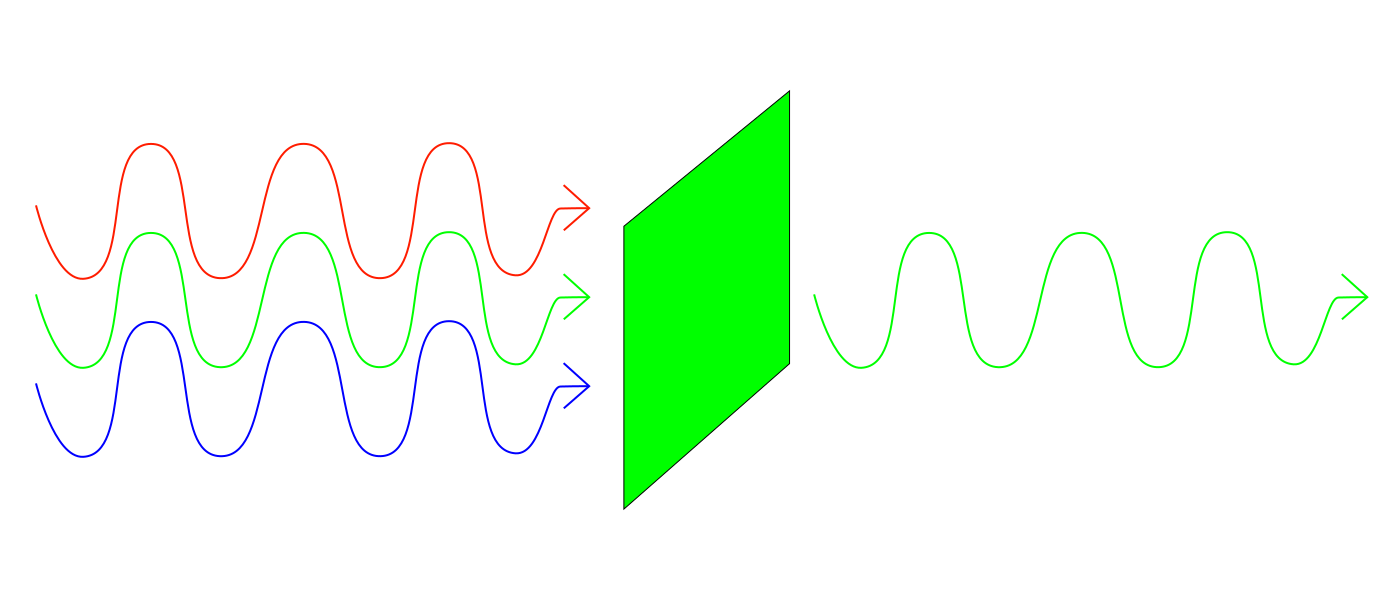
\includegraphics[width=.7\textwidth]{images/substractive_color_mixing.png}
    \end{center}
    \caption{Prinzip subtraktive Farbmischung mit einem Farbfilter}
\end{figure}
\noindent
Eine wahrgenommen Farbe, oder ein Farbton wird auch Farbvalenz genannt. Verschiedene spektrale Zusammensetzungen von Licht können die gleiche Farbvalenz besitzen.
"'Die Menge der möglichen Farbempfindungen ist wesentlich kleiner als die der sie erzeugenden spektralen Verteilungen. Oder anders ausgedrückt: eine Farbvalenz
kann durch viele Farbreizfunktionen $\phi_\lambda$ ausgedrückt werden."'\cite[63]{lichtquellen}
\clearpage

%%%%%%%%%%%%%%%%%%%%%%%%%% Menschliches Farbsehen %%%%%%%%%%%%%%%%%%%%%%%%%%%%%%%%%%%%%%%%%%%%%%%%%%%%%
\section{Menschliches Farbsehen}
Das menschliche Auge besitzt zwei Arten von "'Sensoren"', oder auch Rezeptoren. Stäbchen zur Helligkeitswahrnehmung bei Nacht und
Zapfen zur Helligkeits- und Farbwahrnehmung bei Tag. Das Verhältnis von Zapfen zu Stäbchen beträgt im Schnitt 20:1.\\
Somit ist das Sehen bei Tag ca. sieben Mal so hoch aufgelöst wie bei Nacht.
\begin{figure}[H]
    \begin{center}
        
\includegraphics[width=.8\textwidth]{images/eye.png}
    \end{center}
    \caption{Schematische Darstellung des Auges \cite{wisotopTriChro}}\label{fig:eye}
\end{figure}
\noindent
Ähnlich wie verschiedene Photodioden, welche einzelne Spektralbereiche abdecken, decken auch die Zapfen nur einen
bestimmten Bereich im Farbspektrum ab. Es gibt drei verschiedene Arten von Zapfen. S-, M-, und L-Zapfen. Also "'Short"',
"'Middle"' und "'Long"' Zapfen. Die Längenangaben beziehen sich auf den Wellenlängenbereich, auf welchen die Zapfen
resistiv sind.\\
\begin{figure}[H]
    \begin{center}
        \includegraphics[width=.8\textwidth]{images/eye_spectrum.png}
    \end{center}
    \caption{Darstellung des sichtbaren Farbspektrums der Zapfen des Auges}\label{fig:eye_spectrum}
\end{figure}
\noindent
Die Mengenverteilung der verschiedenen Zapfenarten liegt circa bei S:M:L 1:16:32. Stäbchen und Zapfen übergeben die
empfangen Farbreize and den Sehnerv. Dieser leitet die Informationen an das Gehirn weiter.
\clearpage

%%%%%%%%%%%%%%%%%%%%%%%%%% Farbräume %%%%%%%%%%%%%%%%%%%%%%%%%%%%%%%%%%%%%%%%%%%%%%%%%%%%%%%%%%%%%%%%%%
\section{Farbräume}
\subsection{Farbspektrum}
Wie bereits in \ref{light and measurement} beschrieben ist das Farbspektrum die Entsprechung des Wahrnehmungsbereiches des menschlichen
Auges im elektromagnetischen Spektrum. Das Farbspektrum ist kein Farbraum, da hier keine Mischfarben wie Pink auftreten. Jedoch ist besonders
in dieser Arbeit das Farbspektrum die Referenz für die weiteren Berechnungen in die genutzten Farbräume.
\begin{figure}[H]
    \includegraphics[width=\textwidth]{images/farbspektrum.png}
    \caption{Darstellung des sichtbaren Farbspektrums \cite{fhtEsslignen}}
\end{figure}
\noindent
\subsection{Graßmannsche Gesetze}
"'Hermann Günther Graßmann war ein deutscher Mathematiker, Physiker und Sprachwissenschaftler. Er gilt als eigentlicher Begründer der
Vektorrechnung."'\\\cite{wikipediaGrassmann}\\
"'Die von Graßmann aufgestellten Gesetze bezogen sich weitestgehend auf die additive Farbmischung, gelten aber auch grundlegend bei der
subtraktiven Farbmischung. ... Ganz allgemein erlaubt diese Lehre von den Maßbezeichnungen der Farben eine Beschreibung der Farbvalenz
mit grafischen Mitteln, ... auf einem Diagramm der graßmannschen Farbmischungsberechnung mit Hilfe von Vektoren dargestellt ist. Diese
Art der Berechnung geht ebenfalls fundamental auf die Arbeiten Graßmanns zurück."'\\\cite{wikipediaGrassmannGestze}\\
\\
Erstes graßmannsches Gesetz:\\
"'Jeder Farbeindruck kann mit genau drei Grundgrößen vollständig beschrieben werden.
\begin{align}\label{Equ:2}
    \{C\} \equiv R.\{R\} + G.\{G\} + B.\{B\} \textrm{\hspace{1em} bzw. \hspace{1em}} \{C\} \equiv \left[ \begin{array}{r}
        R \\
        G \\
        B \\
    \end{array}\right]
\end{align}
"'\cite{wikipediaGrassmannGestze}\\
\\
Zweites graßmannsches Gesetz:\\
"'Mischt man eine Farbe mit sich veränderndem Farbton mit einer Farbe, bei der der Farbton immer gleich bleibt, so entstehen Farben mit
sich veränderndem Farbton, wie es durch die Schnittmengen der Farbflächen im Begleitbild illustriert wird.
\begin{align}\label{Equ:3}
    \textrm{Zwei Farben, \hspace{.5em}} \{C_1\} \equiv \left[ \begin{array}{r}
        R_1 \\
        G_1 \\
        B_1 \\
    \end{array}\right]
    \textrm{\hspace{.5em} und \hspace{.5em}} \{C_2\} \equiv \left[ \begin{array}{r}
        R_2 \\
        G_2 \\
        B_2 \\
    \end{array}\right]
\end{align}
ergeben nach additiver Farbmischung die Farbe
\begin{align}\label{Equ:4}
    \{C\} \equiv \{C_1\} +\{C_2\} \equiv \left[ \begin{array}{r}
        R_1 + R_2 \\
        G_1 + G_2 \\
        B_1 + B_2 \\
    \end{array}\right]
\end{align}
Hiermit beschreibt Graßmann im Prinzip die (mathematische) Homogenität des Farbraumes – egal welche Farbtonveränderung man an einer Farbe
vornimmt, das Mischprodukt folgt analog."'\cite{wikipediaGrassmannGestze}\\
\\
Drittes graßmannsches Gesetz:\\
"'Der Farbton einer durch additive Farbmischung entstandenen Farbe hängt nur vom Farbeindruck der Ausgangsfarben, nicht jedoch von deren
physikalischen (spektralen) Zusammensetzungen ab. ...
\begin{align}\label{Equ:5}
    \{C'\} \equiv k.\{C\} \equiv \left[ \begin{array}{r}
        k.R \\
        k.G \\
        k.B \\
    \end{array}\right]
\end{align}
Dieses Gesetz besagt, dass das Mischverhalten selbst der metameren Farben – also derjenigen Farben mit gleichem Farbeindruck, aber
zugleich unterschiedlicher spektraler Zusammensetzung – rein aufgrund ihres Farbeindruckes exakt beschrieben werden kann. Umgekehrt können
also vom Mischverhalten her keine unmittelbaren Rückschlüsse auf die spektrale Zusammensetzung einer Farbe gezogen werden."'\\
\cite{wikipediaGrassmannGestze}\\
\\
Viertes graßmannsches Gesetz:\\
"'Die Intensität (bzw. Totalintensität) einer additiv gemischten Farbe (T3) entspricht der Summe der Intensitäten der Ausgangsfarben ...
\begin{align}\label{Equ:6}
    T(A+B) \equiv T(A) + T(B)
\end{align}
Laut David L. MacAdam gilt dieses Gesetz nur für den Spezialfall einer idealisierten, auf einen Punkt reduzierten Quelle, nicht aber für
ausgedehntere Farbflächen. Graßmann hatte sich nur mit dem oben genannten Spezialfall befasst."' \cite{wikipediaGrassmannGestze}\\
\\
Die hier aufgeführten Gesetze von Graßmann bilden die Grundlage für alle Berechnungen von Koordinaten innerhalb eines Farbraumes. Alle folgenden
Berechnungen dieser Arbeit stützen sich auf diese Gesetze. "'Die von Graßmann aufgestellten Gesetze wurden lange Jahre in der wissenschaftlichen
Welt so gut wie nicht anerkannt – heute jedoch bilden sie eine weitestgehend immer noch gültige Grundlage aller modernen Farblehren und -räume."'\\
\cite{wikipediaGrassmannGestze}
\subsection{RGB}
Der RGB Farbraum baut auf dem Prinzip der trichormatischen Theorie auf. Diese Theorie wurde maßgeblich von Hermann von Helmholtz um 1890 entwickelt. Sie
beschreibt drei Grundfarben: Rot, Grün und Blau. Helmholtz beobachtete, dass aus drei Farbvalenzen jede beliebige Valenz innerhalb des Gamut
additiv gemischt werden kann. Diese Theorie wurde von Hermann Graßmann weiterentwickelt.\\
Der RGB Farbraum beschreibt mit einem Zahlentripel eine Farbvalenz. Diese Zahlen beschreiben die Intensität von rotem (R), grünen (G) und
blauem (B) Licht. Die Werte für R, G und B sind einheitenlos. Oft werden diese von 0 bis 1 definiert, aber weitere übliche Wertebereiche
von 0 bis 100 Prozent und von 0 bis 255 (8 bit) für digitale Anwendungen werden genutzt. \cite{wikipediaRGB}\\
Grafisch wird der RGB Farbraum in den meisten Publikationen als Würfel in einem kartesischen Koordinatensystem dargestellt. Dieser Würfel
mit einer Kantenlänge von eins umschließt die in diesem Farbraum abbildbaren Farbvalenzen.
\begin{figure}[H]
    \includegraphics[width=\textwidth]{images/rgb_color_cube.png}
    \caption{RGB Farbwürfel \cite{wisotopRGB}}
\end{figure}
\noindent
Bei den Koordinaten (0,0,0) ist Schwarz definiert. Bei (1,1,1) ist der Weißpunkt definiert. Die Graulinie befindet sich auf der Diagonalen
von Schwarz zum Weißpunkt. Ein Grauton besteht daher immer aus einem Zahlentripel eines Wertes. \cite{wisotopRGB}\\
Der RGB Farbraum wird im Allgemeinen bei selbst emittierenden Körpern, welche der additiven Farbmischung unterliegen, angewendet. Heutzutage
wird die RGB Definition noch zur Bildwiedergabe in Monitoren oder zur Farbdefinition in HTML Seiten verwendet.\\
Jedoch bildet der RGB Farbraum nicht alle Farbvalenzen ab, die für das menschliche Auge wahrnehmbar sind. Daher wurde im Jahr 1931 ein erster
Normierungsversuch beschlossen, um ein "'weltweit einheitliches Darstellungssystem zu finden"'.\\\cite{wikipediaRGB}
\subsection{CIE} \label{section_CIE}
"'Das CIE-Normvalenzsystem oder \ac{cie}-Normfarbsystem wurde von der Internationalen Beleuchtungskommission (\ac{cie} – Commission internationale de l’éclairage)
definiert, um eine Relation zwischen der menschlichen Farbwahrnehmung (Farbe) und den physikalischen Ursachen des Farbreizes (Farbvalenz) herzustellen.
Es erfasst die Gesamtheit wahrnehmbarer Farben. Unter Nutzung der Farbraumkoordinaten ist auch die Bezeichnung Yxy-Farbraum oder CIE-Yxy gebräuchlich"'
\cite{wikipediaCIE}\\
Der \ac{cie} Farbraum ersetzt die bekannten drei "'realen"' Grundgrößen Rot, Grün und Blau durch "'imaginäre'" Grundgrößen X, Y und Z. Hier steht aber auch
X für den Rotanteil der Farbvalenz, sowie Y für die grüne und Z für die blaue Valenz. Doch ist dies nicht wie in RGB linear. Die Grundgrößen werden mit
sogenannten Empfindlichkeitskurven beschrieben.
\begin{figure}[H]
    \begin{center}
        \includegraphics[width=.5\textwidth]{images/cie_tristimul.png}
    \end{center}
    \caption{CIE XYZ genormte Empfindlichkeitskurven \cite{wikipediaCIE}}
\end{figure}
\noindent
Hier sind die Kurven, welche auch für das Tristimulus Verfahren benötigt werden, grafisch dargestellt. Bei dem Tristimulus Verfahren werden die spektrale Energie
einer Wellenlänge mit dem korrespondierenden Wert für jeweils X, Y und Z multipliziert, um die CIE XYZ Koordinate zu erhalten.\\
Die Empfindlichkeitskurven ahmen die spektrale Empfindlichkeit des menschlichen Auges nach. X kann auch durch L ersetzt werden für die langwellig sensitiven Zapfen
des Auges. Gleiches gilt für Y mit M und Z mit S. Somit kann man diese Darstellung als LMS-Farbraum bezeichnen.\\
\subsubsection{Standardbeleuchtung} \label{whiteRef}
"'Das CIE-Normvalenzsystem wurde ursprünglich in Hinsicht auf Beleuchtungsfragen entwickelt. Das System erlaubt prinzipiell jede denkbare Kombination an X-, Y-
und Z-Werten. Um eine normierte Übersicht der Farben zu erreichen wurden neutralweiße Normlichtfarben definiert. Aus Gründen der Farbwahrnehmung befinden sich diese
auf der Black-Body-Kurve, da dies mit einer Farbtemperatur verbundene Beleuchtungen sind."' \cite{wikipediaCIE}\\
Dies bedeutet, dass von dem roten Bereich zum Weißpunkt des CIE Diagramms eine Kurve zu finden ist, welche die verschiedenen Farbtemperaturen repräsentiert. Für die Umrechnung
in andere Farbräume, wie zum Beispiel RGB, muss ein Referenzweißpunkt definiert werden wo sich die Weißpunkte der beiden Farbräume decken. Je nach Weißpunkt gibt es 
für die gleiche Umrechnung verschiedene Umrechnungsmatrizen.\\
In dieser Arbeit wird der Weißpunkt D65 als Referenzpunkt genutzt. "'Das Spektrum hat eine ähnlichste Farbtemperatur von 6504 Kelvin. Genutzt wird dieses Normlicht als Weißpunkt für sRGB"' \cite{wikipediaCIE}
\subsubsection{CIE 1931}
Der 1931 definierte \ac{cie} Farbraum, auch umgangsprachlich als "'Schuhsohle"' bezeichnet, wird in der Regel zweidimensional dargestellt. In dem Koordinatensystem
bewegt man sich mit x auf der x-Achse und mit y auf der y-Achse. Zusätzlich wird eine CIE 1931 Koordinate noch mit Y (groß Y) für die Helligkeit der Farbvalenz
beschrieben.
Hier wird in der Regel eine Konstante angenommen mit der Definition des Weißpunktes (siehe \ref{whiteRef}).
\begin{figure}[H]
    \begin{center}
        \includegraphics[width=.7\textwidth]{images/cie_1931.png}
    \end{center}
    \caption{CIE 1931 2D Farbraum \cite{wikipedia1931Image}}
\end{figure}
\noindent
Die xy Koordinaten sind 1 normiert. Außerdem gilt:
\begin{align}
    x + y <= 1
\end{align}
Mit den folgenden Formeln lassen sich die x und y Koordinaten errechnen. Y bleibt als Luminanzfaktor erhalten.
\begin{align}\label{Equ:7}
    x = \frac{X}{X+Y+Z}\\
    y = \frac{Y}{X+Y+Z}\\
    Y = Y \label{Equ:8}
\end{align}
\cite{lindbloom}
\subsubsection{CIE 1976}
Auch der 1976 definierte Farbraum basiert auf den X,Y und Z Werten. Der Farbraum wurde eingeführt, um einen Farbraum mit gleichmäßig verteilteren Farbflächen zu
definieren. In dem ebenfalls zweidimensionalen Koordinatensystem bewegt man sich mit u auf der x-Achse und mit v auf der y-Achse.
\begin{figure}[H]
    \begin{center}
        \includegraphics[width=.7\textwidth]{images/cie_1976.png}
    \end{center}
    \caption{CIE 1976 2D Farbraum \cite{wikipedia1976}}
\end{figure}
\noindent
"'Der CIE LUV-Farbraum ist eine Ableitung des Standard CIE XYZ-Farbraums, in dem der Abstand der Farben dem menschlichen Farbsehen besser entgegenkommt."' \cite{wisotoLuv}
Mit den folgenden Formeln lassen sich die u' und v' Koordinaten errechnen.
\begin{align}\label{Equ:9}
    u' = \frac{4X}{X+15Y+3Z}\\
    v' = \frac{9Y}{X+15Y+3Z}
\end{align}
\cite{lindbloom}\\
Um mehrere Farben zu vergleichen muss die u'v' Koordinate auf ein Referenzweiß ($X_r$,$Y_r$,$Z_r$) bezogen werden. So ergeben sich absolute uv Koordinaten. Die Luminanz
L ist ein Faktor für die Bestimmung der Sättigung $s_{uv}$ der Farbvalenz. \cite{wikipedia1976}
\begin{align}\label{Equ:10}
    &y_r = \frac{Y}{Y_r}\\
    &L = \left\{
        \begin{array}{ll}
            116 \sqrt[3]{y_r} - 16 & \text{if } y_r > \epsilon \\
            \kappa y_r & \text{otherwise}
        \end{array}
        \right.\\
    &u = 13 L (u' - u_r')\\
    &v = 13 L (v' - v_r')\\
    &\epsilon = \left\{
        \begin{array}{ll}
            {0.008856} & \text{Actual CIE standard} \\
            {216 / 24389} & \text{Intent of the CIE standard}
        \end{array}
        \right.\\
    &\kappa = \left\{
        \begin{array}{ll}
            {903.3} & \text{Actual CIE standard} \\
            {24389 / 27} & \text{Intent of the CIE standard}
        \end{array}
        \right.\\
    &s_{uv} = \frac{C^*_{uv}}{L}\\
    &C^*_{uv} = \sqrt{(u^2*v^2)}\\
\end{align}
\cite{lindbloom}, \cite{wikipedia1976}\\
\\
Wenn die uv Koordinaten auf 0 gesetzt werden, also auf dem Referenzweißpunkt liegen variiert L die Grauskala der Valenz. \cite{wisotoLuv}
\clearpage

%%%%%%%%%%%%%%%%%%%%%%%%%% LED %%%%%%%%%%%%%%%%%%%%%%%%%%%%%%%%%%%%%%%%%%%%%%%%%%%%%%%%%%%%%%%%%%%%%%%%%
\section{LED}
\subsection{Allgemein}
\ac{led} ist das Acronym für Light Emitting Diode, also lichtemittierende Diode. Dies ist eine spezielle Art von Halbleitern,
welche bei einem Stromfluss Licht emittieren. Die chemische Zusammensetzung (Dotierung) der Diode entscheidet, welche Farbe
beziehungsweise welche Frequenz sie emittiert.\\
Im Folgenden ein Auszug der Element-Farbzuordnung \cite{wikiLed}:
\begin{table}[H]
    \small
    \begin{tabular*}{\textwidth}{l @{\extracolsep{\fill}} ll}
        Element & Farbe & Wellenlänge (nm)\\
        Aluminiumgalliumarsenid (AIGaAs) & Rot, Infrarot & 665 - 1000\\
        Galliumarsenidphosphid (GaAsP) & Rot, Orange und Gelb & 570 - 760\\
        Galliumphosphid (GaP) & (Gelb-)Grün & 500 - 580\\
        Indiumgalliumnitrid (InGaN) &  Grün, Blau, Violett und Ultraviolett & 520 - 230\\
    \end{tabular*}
\end{table}
\noindent
Zunächst wurden \ac{led}s in den frühen 1960er Jahren als Leuchtindikatoren benutzt. Also zum Beispiel auf
Platinen als Statusanzeige oder wie wir es heute von vielen Ethernetanschlussbuchsen kennen als blinkende Anzeige, die den Datenempfang
signalisiert. Durch die voranschreitende technische Entwicklung der \ac{led}, wie bessere Effizienz und bessere Lichtausbeute, sowie verbesserter
Langlebigkeit des Bauteils, fand anfang der 1990er die \ac{led} auch ihre Anwendung im Heimbereich.\\
\ac{led}s "'emittieren Licht in einem begrenzten Spektralbereich. Das Licht ist nahezu monochromatisch. Deshalb sind sie beim Einsatz als
Signallicht besonders effizient im Vergleich zu anderen Lichtquellen, bei denen zur Erzielung einer monochromen Farbcharakteristik
Farbfilter den größten Teil des Spektrums absorbieren müssen."'\\
\cite{wikiLed}

\subsection{Mischen von Farben}\label{colormixing}
Emittierende Körper unterliegen der additiven Farbmischung. Dies bedeutet, dass sich die ins elektromagnetische Spektrum abgegebenen
Wellen bei ihren jeweiligen Wellenlängen aufaddieren. Somit kann mit verschiedenen LED Lichtquellen eine neue Farbe gemischt
werden.\\
So kann beispielsweise mit einer roten und einer grünen \ac{led} ein orangener bis gelber Farbton gemischt werden.

\subsection{Weiße LEDs}
Eine tatsächlich weiße \ac{led} existiert bisher auf dem Markt nicht, da \ac{led}s generell schmalbandig abstrahlen. Die heutzutage
verwendeten "'weißen"' \ac{led}s sind eigentlich blaue \ac{led}s, mit einem zusätzlichen Phosphor Filter als breitbandigem Lumineszenzfarbstoff.
\begin{figure}[H]
    \centering
    \begin{subfigure}[b]{0.49\textwidth}
        \includegraphics[width=\textwidth]{images/LED_weiss_P_blau.png}
        \caption{Funktionelles Blockdiagramm}
    \end{subfigure}
    \hfill 
    \begin{subfigure}[b]{0.49\textwidth}
        \includegraphics[width=\textwidth]{images/LED_weiss_phosphor.png}
        \caption{Spektrale Abdeckung}
    \end{subfigure}
    \caption{Weiße LED - Aufbau und Spektrum \cite{wikiLed}}\label{fig:White LED}
\end{figure}
\noindent
Dies verschiebt das abgestrahlte Licht in den gelben Bereich. Somit entsteht mit einem Teil des blauen Lichts und mit dem farbverschobenen Spektrum
ein breitbandiges Abstrahlverhalten.
\clearpage

%%%%%%%%%%%%%%%%%%%%%%%%%% Lichtquellen in der Veranstaltungstechnik %%%%%%%%%%%%%%%%%%%%%%%%%%%%%%%%%%%%%%%%%%%
\section{Lichtquellen in der Veranstaltungstechnik}
Für die Veranstaltungstechnik ist künstliches Licht nahezu unverzichtbar. Von der Grundausleuchtung in einem Theater bis zum Effektlicht
auf Kleinveranstaltungen. In den frühen Jahren der großen Konzerte wurde die Bühne hauptsächlich mit Scheinwerfern mit Glühfaden Leuchtmitteln beleuchtet.
Diese Form der Beleuchtung wurde in der Veranstaltungstechnik als Kunstlicht bezeichnet.\\
Weiter werden vornehmlich in Theatern, sowie Film- und Fernseherproduktion Tageslichtscheinwerfer benutzt. Tageslichtleuchtmittel
unterscheiden sich von der Art der Lichterzeugung gegenüber Glühlicht. Hier kommen anstatt eines Glühfadens zwei Elektroden in einer
gasgefüllten Röhre zum Einsatz. Mit dem Anlegen einer Spannung an den beiden Elektroden baut sich ein elektrisches Feld auf, welches zu
einer Gasentladung und somit zu einer Lichtemittierung führt. Solche Gasentladungslampen oder auch \ac{hmi} (Halogen-Metalldampflampe)
werden für diese Anwendungen in der Regel mit Xenon befüllt. Das emittierte Licht ist ähnlich dem Spektrum des Sonnenlichtes auf der
Erde. Daher der Name Tageslichtscheinwerfer.
\begin{figure}[H]
    \centering
    \begin{subfigure}[b]{0.49\textwidth}
        \includegraphics[width=\textwidth]{images/conventional_spectrum.png}
        \caption{Glühlichtlampe}
    \end{subfigure}
    \hfill 
    \begin{subfigure}[b]{0.49\textwidth}
        \includegraphics[width=\textwidth]{images/HMI_Spectrum.png}
        \caption{Gasentladungslampe}
    \end{subfigure}
    \caption{Typische Spektren der verschiedenen Leuchtmittel\cite{showlicht}[35+37]}\label{fig:lightEmiiterSpects}
\end{figure}
\noindent
In den 2000er Jahren hielt dann die LED Einzug in die Welt der Veranstaltungstechnik. Damit begann ein Wandel besonders im Bezug auf die Lebensdauer
der Leuchtmittel und der Lichtausbeute im Vergleich zum Stromverbrauch. Mit der fortschreitenden Entwicklung der \ac{led} und der
Scheinwerfer, welche diese nutzen, hat die \ac{led} heute an vielen Stellen die konventionelle Glühlampe oder \ac{hmi} verdrängt.\\
Die Lebensdauer einer auf \ac{led}-Technik basierenden Lampe liegt im Bereich von 15.000 bis 45.000 Betriebsstunden. Eine Glühlampe hingegen
hat nur eine Lebensdauer von etwa 300 Betriebstunden. Eine Gasentladungslampe hält eine Betriebsbelastung von etwa 300 bis 2000 Stunden aus.
Eine weitere Stärke der LED ist der niedrige Stromverbrauch bei einer vergleichbaren Lichtausbeute gegenüber einer Glühlampe oder \ac{hmi}.
Ein PAR64 Medium Flood CP62 hat eine Lichtausbeute von etwa 320 Lumen mit einer Leistung von 1000 Watt \cite{convpar}. Ein vergleichbarer moderner
\ac{led} \ac{par} mit einer LED Leistung von 180 Watt hat eine Lichtausbeute von etwa 5100 Lumen \cite{ledpar}. So können heute umfangreichere
Lichtinstallationen umgesetzt werden. Da die verfügbare Leistung an Veranstaltungsorten begrenzt ist, konnte nur eine vergleichsweise geringe
Anzahl von konventionellen \ac{par} Scheinwerfern eingesetzt werden, da schon mit 100 \ac{par}s mit 1000 Watt Anschlussleistung bereits
100.000 Watt zur Verfügung stehen müssten, um alle zur gleichen Zeit zu betreiben. Dies war in der Regel nicht der Fall. Dennoch wurden in der
Vergangenheit bei Großveranstaltungen solche Stückzahlen in Bühnen verbaut und dies nicht als einziger Scheinwerfertyp.
Denn hier hat die LED einen weiteren Vorteil zu damals.\\
Früher wurden um eine Bühne in verschiedenen Farben auszuleuchten mehrere \ac{par}s benötigt. Um nur rot, grün, blau und weiß leuchten zu
können, benötigte man vier \ac{par}s. Drei davon mit einer jeweiligen Farbfolie vor dem Lichtaustritt. Farbfolien nutzen das Konzept der
subtraktiven Farbmischung. Es werden vor eine in der Regel weiße Lichtquelle hitzebeständige Folien gespannt, welche nur bestimmte Teile des 
Lichtspektrums durchlassen.\\
Dadurch war die Gesamtleistung aller eingesetzten Scheinwerfer früher deutlich größer als dem Licht für die Veranstaltung zugedacht war. Doch
da die Lampen für die verschieden Farben nie alle zur gleichen Zeit an waren, war dies nur ein Problem im Haushalten mit der zur verfügungstehenden
Leistung.\\
Mit \ac{led} Scheinwerfern gibt es dieses Problem heute kaum mehr. Die Scheinwerfer können durch das Verbauen von mehrfarbigen \ac{led}s (siehe
\ref{colormixing}) in einem \ac{led} \ac{par} mit additiver Farbmischung ein großes Repertoire an Farben bereitstellen.
Dennoch sind die Traversen auf den Großveranstaltungen voller geworden gegenüber früher.
Die ersten \ac{led} \ac{par}s hatten viele einzelne rote, grüne und blaue 5-mm-\ac{led}s. Hier war jedoch das Problem, dass bei der Farbmischung
mit beispielsweise Rot und Grün kein homogenes Gelb entstanden ist, da jede einzelne \ac{led}s ihr eigenes Streuverhalten hatte. So konnte
auf einer auftreffenden Fläche wie dem Boden immer einzelne nur rote oder nur grüne Farbflächen entstehen. Dieses unerwünschte Verhalten wurde
später gelöst, indem mehrere \ac{led}s in einen Chip integriert wurden, und vor jeden dieser \ac{led}-Chips eine Streulinse gesetzt wurde.
Somit konnte ein deutlich homogeneres Abstrahlverhalten erreicht werden.
\clearpage

%%%%%%%%%%%%%%%%%%%%%%%%%% Verwendete Geräte %%%%%%%%%%%%%%%%%%%%%%%%%%%%%%%%%%%%%%%%%%%%%%%%%%%%%%%%%%%%%%%%%%%%
\section{Verwendete Geräte}
\subsection{Lampen}
Im Folgenden werden die Lichtquellen beziehungsweise die Lampen beschrieben, die für die Messungen verwendet wurden.
Auch in der Veranstaltungstechnik als (engl.) "'Fixtures"' bezeichnet. Diese Lampen haben alle \ac{led}s als Lichtquelle. Diese \ac{led}s
sind alle unterschiedlich aufgebaut.
\subsubsection{Ape Labs Light Can}
~\par\vspace{-\baselineskip}
\begin{wrapfigure}{r}{0.4\textwidth}
    \vspace{-45pt}
    \begin{center}
        \includegraphics[width=.23\textwidth]{images/light_can_front.png}
    \end{center}
    \vspace{-20pt}
    \begin{center}
        \caption{Light Can\\\cite{lightCan}}
    \end{center}
    \vspace{-15pt}
\end{wrapfigure}
\noindent
Diese Lampe ist eine sehr kompakt gebaute RGBW \ac{led} Lichtquelle auf Akku Basis. Diese wurde von der Firma Ape Labs aus Eisigen in Deutschland
entwickelt. Diese Lampe ist sowohl per Fernbedienung, als auch per W-\ac{dmx} steuerbar.
Die "'Kanne"' hat einen Abstrahlwinkel von 65 Grad. Zur gezielten Steuerung, ohne vorprogrammierte Effekte wird ein \ac{dmx} zu W-DMX Wandler der
Firma benötigt (W-APP). Dieser ermöglicht dann die Ansteuerung der Lampe durch die Applikation.
\subsubsection{Robe LEDWash 300}
Dieses Wash Movinglight ist ein handelsübliches Gerät und wird weltweit bei vielen Veranstaltungen universell eingesetzt. Hier sind 19 einzelne
RGBW \ac{led}s hinter einzelnen Linsen in zwei Kreisen und einer Mittelpunkt \ac{led} positioniert.
\begin{figure}[H]
    \begin{center}
        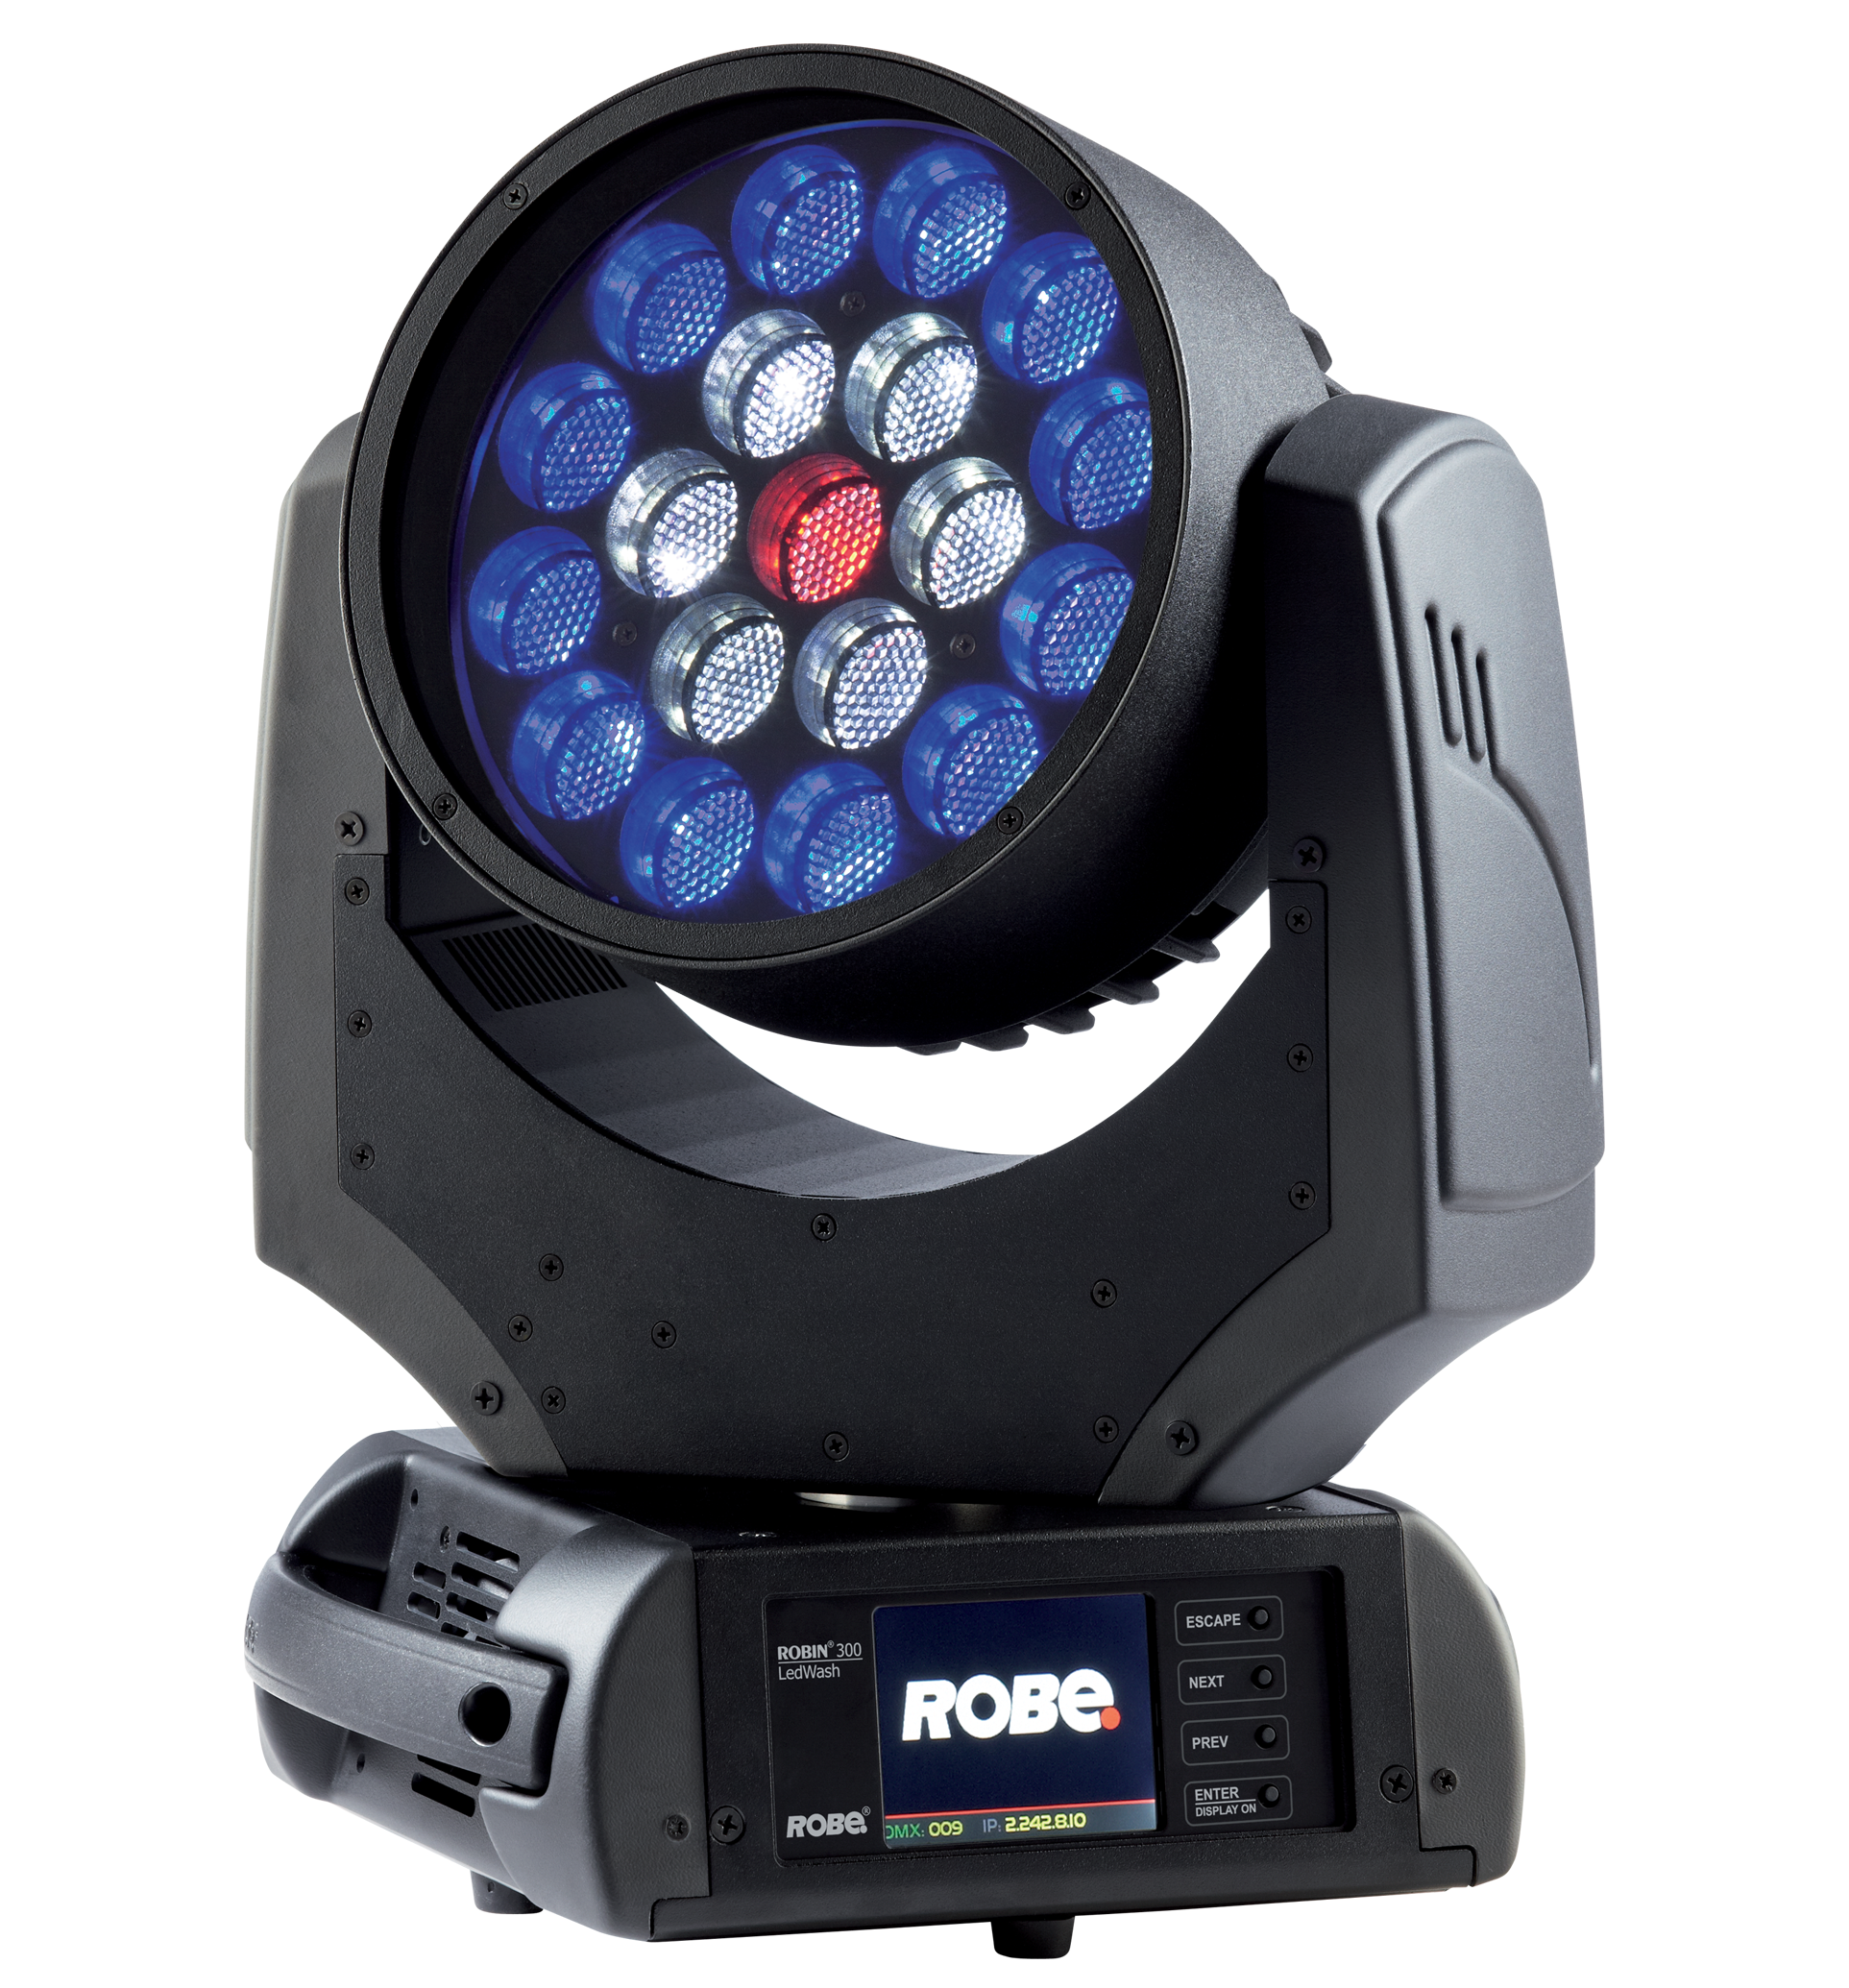
\includegraphics[width=.3\textwidth]{images/Robe_300_ledwash.png}
    \end{center}
    \caption{Robe LEDWash 300 \cite{robe}}
\end{figure}
\noindent
Das Movinglight hat einen einstellbaren Abstrahlwinkel von 8 bis 63 Grad. Dieser wurde allerdings bei den Messungen auf 63 Grad fest eingestellt,
um ein möglichst homogenes Abstrahlverhalten zu erhalten. Laut Hersteller hat die Lampe bei einer Distanz von fünf Metern zur Lampe eine
Lichtausbeute von 3.370 Lumen. Die Lampe ist per \ac{xlr} mit DMX, oder via Ethernet RJ45-Buchse per Art-Net steuerbar. An einem Display
am Fuß (der "'Base"') kann der Scheinwerfer konfiguriert werden.
\subsubsection{ARRI SkyPanel}
Das Skypanel S60-C von der Firma Arri, ein Tochterunternehmen der Firma Osram, wird oft als Fluter, das Grundlicht in Film und Fernsehen, eingesetzt.
Es wird beworben, dass es mit \ac{cie} 1931 xyY Werten per DMX angesteuert werden kann und diese \ac{cie} Werte von der Lampe exakt wiedergegeben werden. Somit
ist diese Lampe eine perfekte Referenz für diese Arbeit.
\begin{figure}[H]
    \begin{center}
        \includegraphics[width=.48\textwidth]{images/skypanel_s60_c.png}
    \end{center}
    \caption{ARRI Skypanel S60-C \cite{arri}}
\end{figure}
\noindent
Das SkyPanel hat einen Abstrahlwinkel von 115 Grad. Die RGBW \ac{led}s befinden sich hinter einem lampengroßem Diffusor. Die Lampe ist per
\ac{xlr} mit DMX, W-DMX oder via Ethernet RJ45-Buchse per Art-Net steuerbar. An einem Display auf der Rückseite kann der Scheinwerfer konfiguriert
werden. Außerdem kann manuell am Gerät auch eine xyY \ac{cie} Farbe ohne externe Ansteuerung eingestellt werden.\\
Bei einer Ansteuerung per DMX oder Art-Net kann am Gerät auch abgelesen werden, welche xyY Werte das Gerät aus der Ansteuerung ermittelt,
und versucht zu emittieren.
\subsection{Messgerät MK350 LED}
Als Referenz Messgerät zu dem vergleichsweisen niedrigpreisigen Sensoren wurde das bei MA Lighting bereits vorhandene Spektralmessgerät
"'MK350 LED"' der Firma UPRtek genutzt.\\
\begin{figure}[H]
    \centering
    \begin{subfigure}[b]{0.49\textwidth}
        \includegraphics[width=\textwidth]{images/MK350N_Basic_Handheld_Spectrometer.png}
        \caption{Produkt \cite{uprtek}}
    \end{subfigure}
    \hfill 
    \begin{subfigure}[b]{0.49\textwidth}
        \includegraphics[width=\textwidth]{images/mk350_lightcan_green.JPG}
        \caption{Grafische Benutzeroberfläche}
    \end{subfigure}
    \caption{UPRtek MK350 LED}
\end{figure}
\noindent
Dieses Messgerät kann Spektraldaten im Bereich von 360 bis 760 Nanometern messen. Hier wird ein Messwert pro einem Nanometer erfasst. Daraus berechnet
das Messgerät die \ac{cie} 1931 xy Koordinaten, sowie die \ac{cie} 1976 uv Koordinaten. Messwerte können einzeln oder auch in Serie erfasst werden und
im CSV Format für die weitere Auswertung auf eine SD Karte gesichert werden.
\clearpage

%%%%%%%%%%%%%%%%%%%%%%%%%% Sensorik %%%%%%%%%%%%%%%%%%%%%%%%%%%%%%%%%%%%%%%%%%%%%%%%%%%%%%%%%%%%%%%%%%
\section{Sensorik}
Es gibt einige Hersteller von entsprechenden Spektralsensoren für Licht und spektral benachbarte Bereiche wie Infrarot.
Ein Hersteller, dessen Sensoren in dieser Arbeit vornehmlich genutzt wurden, ist die Firma AMS.\\
AMS ist ein globales Unternehmen und einer der führenden Hersteller für Sensortechnik. AMS stellt hauptsächlich Sensoren für die Bereiche
Optik, Bildverarbeitungund Schall her. Sensoren von AMS werden in Smartphones und Smarthome Produkten sowie in industrieller Automatisierung
und medizinischen Geräten zu finden. \cite{ams}\\
Zu Beginn wurde nach einer einfachen Evaluierungslösung für das Erfassen von spektralen Daten gesucht. Hier wurde das
Sensorboard von der Firma Adafruit AS7262 genutzt. \cite{adafruit}\\
Dieses Board nutzt einen AMS AS7262 Visible Spectral Light Sensor. Weiter stellt es Pin outs für \ac{i2c} und \ac{uart} bereit,
sowie eine Status-\ac{led} und eine Referenz \ac{led} Weißlichtquelle zur Beleuchtung von nicht selbst emittierenden Gegenständen.
\begin{figure}[H]
    \begin{center}
        \includegraphics[width=.48\textwidth]{images/AS7262_front.png}
    \end{center}
    \caption{Adafruit AS7262 Sensorboard \cite{adafruit}}
\end{figure}
\noindent
Für eine erste Evaluierung und auch für das weitere Vorgehen wurde die UART Schnittstelle genutzt, da diese in der Kommunikation
transparenter aufgebaut ist.\\
Hier ist zu beachten, dass auf dem Adafruit Sensorboard die Lötbrücke für "'\ac{uart} SELECT"' geschlossen werden muss. Ohne diese
Anpassung verbleibt der Chip im \ac{i2c} Modus.\\
Das Sensorboard wurde mit einem "'FTDI Friend"', einem weiteren Produkt von Adafruit, mit dem Endgerät, einem Windows Computer, verbunden.
Dies ist ein USB-Seriell-Transceiver. Dieser Chip von der Firma FTDI wandelt \ac{usb} zu RS232 Analogsignalen. Die Verbindung mit dem \ac{ic}
wird über \ac{uart} via RS232 hergestellt, mit einer Baud Rate von 115200.\\
Die Kommunikation über \ac{uart} mit allen AMS Sensoren funktioniert mit AT-Kommandos, einer \ac{ascii} basierten Kommandosprache,
welche für Modems in den 1980er Jahren entwickelt wurde.
\subsection{AS7261}
Das Sensorspektrum des 7261 ähnelt sehr der Farbreizverarbeitung im menschlichen Auge. Die in Bild \ref{fig:AS7261_spectrum} gezeigte
Gewichtung der Sensoren ist angelehnt an die \ac{cie} 1931 Gewichtungskurven für das menschliche Auge.
\begin{figure}[H]
    \centering
    \begin{subfigure}[b]{0.49\textwidth}
        \includegraphics[width=\textwidth]{images/AS7261_functional_blockdiagram.png}
        \caption{Funktionelles Blockdiagramm}
    \end{subfigure}
    \hfill 
    \begin{subfigure}[b]{0.49\textwidth}
        \includegraphics[width=\textwidth]{images/AS7261_spectrum.png}
        \caption{Spektrale Abdeckung}\label{fig:AS7261_spectrum}
    \end{subfigure}
    \caption{AMS AS7261 \cite{datasheet61}}\label{fig:AS7261}
\end{figure}
\noindent
Neben den \ac{cie} X, Y und Z Sensoren verfügt der Sensor noch über einen \ac{nir}, einen Dark und einen Clear Sensor. Diese finden hier
allerdings keine Verwendung.\\
Die AT Schnittstelle stellt verschiedenste Informationen zur Verfügung. Zunächst kann mit dem Befehl "'ATDATA"' die Sensorwerte als
16-Bit Integer (Ganzzahl) Werte von 0 bis 65535 ausgegeben.\\
\\
Weiter gibt es nicht (spektral) Sensor bezogene Einstellungen die über die \ac{uart} Schnittstelle abgefragt und gesetzt werden können.
Als ein Beispiel kann die Temperatur des Chips in Celsius des \ac{ic}s mit "'ATTEMP"' abgefragt werden.\\
Mit "'ATLED0=100"' kann eine kleine grüne Status \ac{led} angeschaltet werden, um zu signalisieren, dass das Programm eine Verbindung mit 
dem Chip herstellen konnte und die Kommunikation funktioniert.\\
Zusätzlich kann mit den Befehlen "'ATLED1=0"' und "'ATLED1=100"' eine auf dem Evaluationsboard angebrachte weiße Referenz \ac{led} aus und
an geschaltet werden, um nicht selbst emittierende Objekte zu vermessen.\\
Die Schnittstelle stellt noch einige weitere Informationen zur Verfügung, wie die Chip Software-Version, einen Sensor Gain, Sensor Bank Modus
und Integrationszeit.
\subsection{AS7262}
Auch das Sensorspektrum des 7262 ähnelt sehr der Zapfenverteilung im menschlichen Auge. Dieser \ac{ic} hat insgesamt 6 einzelne Photodioden.
Davon sind 4 im rot bis gelbgrünen Teil des Spektrums angesiedelt. Eine weitere Photodiode im grünen Spektralbereich und die letzte im blauen
Bereich. So sind auch in Bild \ref{fig:eye_spectrum} zwei der drei Zapfen Arten im rot bis grünen Bereich. Die dritte Zapfenart ist im blauen
Bereich.
\begin{figure}[H]
    \centering
    \begin{subfigure}[b]{0.49\textwidth}
        \includegraphics[width=\textwidth]{images/AS7262_functional_blockdiagram.png}
        \caption{Funktionelles Blockdiagramm}
    \end{subfigure}
    \hfill 
    \begin{subfigure}[b]{0.49\textwidth}
        \includegraphics[width=\textwidth]{images/AS7262_spectrum.png}
        \caption{Spektrale Abdeckung}\label{fig:spec_7262}
    \end{subfigure}
    \caption{AMS AS7262 \cite{datasheet62}}\label{fig:AS7262}
\end{figure}
\noindent
Hier werden aus der \ac{uart} (AT) Schnittstelle mit dem Befehl "'ATCDATA"' die Sensorwerte der einzelnen Dioden als 32-Bit floating point
(Gleitkomma Zahlen) ausgegeben. Die weiteren nicht Sensor bezogenen Befehle sind identisch mit dem Befehlssatz des AS7261 Sensors.
\clearpage

%%%%%%%%%%%%%%%%%%%%%%%%%% Messungen %%%%%%%%%%%%%%%%%%%%%%%%%%%%%%%%%%%%%%%%%%%%%%%%%%%%%%%%%%%%%%%%%
\section{Messungen und Testapplikation}
\subsection{Empfangen und Aufbereiten der Sensorwerte}
\subsubsection{Erfassen der Messwerte mit dem AS7262}
Zu Beginn wurde der Sensor AS7262 in Betrieb genommen, da dieser auf einem Evaluierungsboard verfügbar war.
Zunächst wurden mit der Applikation "'Putty"' über die COM Schnittstelle einige Kommandos gesendet, um die
\ac{uart} Schnittstelle zu testen. Dies ist erfolgreich gelungen. Es wurden erste spektrale Werte des
Umgebungslichtes und einer Light Can empfangen. Es wurde der Befehl "'ATDATA"' genutzt.\\
Anschließend wurde damit begonnen, eine erste NodeJS Applikation zu programmieren, um intervallweise spektrale Daten
von der \ac{uart} Schnittstelle abzufragen und anzuzeigen. So konnten erste Messwerte mit dem AS7262 Sensor erhoben werden.
Diese Messwerte wurden mit dem MK350 verglichen. Hier wurde beobachtet, dass die gemessenen Daten des MK350 auf den jeweiligen
Wellenlängen mit den Werten übereinstimmen. Hier ist anzumerken, dass - wie in Bild \ref{fig:green_spec_MK350} zu sehen - die pro Wellenlänge
gemessene Amplitude nach 1 normiert wird. Zur Vergleichbarkeit werden auch in der Applikation die Sensor Werte des AS7262 nach
1 normiert. Die Messwerte der sechs Wellenlängen des AS7262 sind mit geringer Abweichung identisch zum MK350.\\
\begin{figure}[H]
    \centering
    \begin{subfigure}[b]{0.49\textwidth}
        \includegraphics[width=\textwidth]{images/mk350_lightcan_green_spectrum.png}
        \caption{Spektrum MK350}\label{fig:green_spec_MK350}
    \end{subfigure}
    \hfill 
    \begin{subfigure}[b]{0.49\textwidth}
        \includegraphics[width=\textwidth]{images/app_lightcan_green_spectrum.png}
        \caption{Spektrum AS7262}\label{fig:green_spec_7262}
    \end{subfigure}
    \caption{Spektrum des grünen Emitters einer LightCan. Gemessen am 10.09.2019}
\end{figure}
\noindent
Doch war hier ein großes Defizit des AS7262 zu beobachten. Wie in Bild  \ref{fig:green_spec_MK350} zu erkennen liegt das Maximum
des grünen Emitters bei ca. 515 Nanometern. Doch liegen die beiden nächsten Messflanken des AS7262 bei 500 und 550 Nanometern (Bild \ref{fig:spec_7262}).
Somit wird der Wellenlängenbereich mit der höchsten Energiedichte nicht erfasst. Dies erzeugt eine relevante Fehlerquelle für weitere
Berechnungen.\\
Nach der Implementierung der ersten Auswertung der Messdaten eines mit der Applikation verbundenen Sensors wurde begonnen, die Messwerte in der
Applikation grafisch aufzubereiten. Zunächst wurde die NodeJS mit dem \ac{npm} Paket Electron erweitert. Auf der Appcode Seite ist ein Befehlssatz
zur Generierung eines Electron Fensters, sowie eine Abfrage des Sensors mit dem Befehl "'ATCDATA"', welcher intervallweise alle 250 Millisekunden
abgerufen wird. Die empfangenen Sensordaten werden dann per Schnittstelle an den Webcode weitergegeben.\\
Mit den im Webcode verfügbaren Sensordaten wurden in Anlehnung zu der Darstellung im MK350 die Werte mit proportional hohen Balken pro Wellenlänge
mit HTML Elementen dargestellt. Diese Balken wurden zur besseren Zuordnung in eine, die Wellenlänge repräsentierende, Farbe eingefärbt.
\begin{figure}[H]
    \begin{center}
        \includegraphics[width=.6\textwidth]{images/app_dummy_spectrum.png}
    \end{center}
    \caption{Erste Darstellung der Sensorwerte}
\end{figure}
\noindent
Die 1 normierten Werte bezogen auf den maximal gemessenen einheitlosen Wert sind unter den Balken angezeigt. Der gemessene Maximalwert wird in der
oberen linken Ecke angezeigt. Unter den normierten Messwerten ist zusätzlich ein beschreibender Name der Farbe, sowie die Wellenlänge aufgeführt.\\
\\
Mit diesen Werten wurde begonnen, eine XYZ \ac{cie} Koordinate zu errechnen. Hier wurden die Formeln von Bruce Lindbloom genutzt. Lindblooms Webauftritt
dient bereits in vielen Büchern und anderen Publikationen als Referenz für Themen wie Farbräume oder Umrechnung zwischen Farbräumen.\\
Zur Umrechnung eines diskreten Farbspektrums zu einer \ac{cie} XYZ Koordinate sind folgende Formeln gegeben \cite{lindbloom}:
\begin{align}\label{Equ:11}
    X = \sum_{i}x_i*P_i\Delta\lambda\\
    Y = \sum_{i}y_i*P_i\Delta\lambda\\
    Z = \sum_{i}z_i*P_i\Delta\lambda
\end{align}
Die Variablen $x_i$, $y_i$ und $z_i$ stehen hier für die Tristimuluskurven (Standard Observer Functions) oder auch Empfindlichkeitskurven aus Kapitel \ref{section_CIE}.
Eine Aufstellung der Tristimuluswerte wurde von der Website "'Wisotop"' von der Fachhochschule Köln entnommen. Die Dokumentationen der
\ac{cie} Kommission sind nicht öffentlich einsehbar.
Die hier genutzten Tristimuluswerte \cite{wisotop}:
\begin{table}[H]
    \small
    \begin{tabular*}{\textwidth}{l @{\extracolsep{\fill}} llllll}
        Wellenlänge & 450 & 500 & 550 & 570 & 600 & 650\\
        X & 0.3362 & 0.0049 & 0.4334 & 0.7621 & 1.0622 & 0.2835\\
        Y & 0.0380 & 0.3230 & 0.9950 & 0.9520 & 0.6310 & 0.1070\\
        Z & 1.7721 & 0.2720 & 0.0087 & 0.0021 & 0.0008 & 0.0000\\
    \end{tabular*}
\end{table}
\noindent
Aus diesen Werten und den mit dem Sensor erfassten Spektralwerten konnten nun die \ac{cie} XYZ Werte errechnet werden.
\begin{figure}[H]
    \begin{center}
        \includegraphics[width=\textwidth]{images/app_dummy_spectrum_with_xy.png}
    \end{center}
    \caption{Darstellung der Sensorwerte und CIE 1931 Diagramm}
\end{figure}
\noindent
\subsubsection{Erfassen der Messwerte mit dem AS7261}
Da der AS7261 nicht als Evaluierungskit von Adafruit verfügbar war, wurde ein zweites 7262 Sensorboard von Adafruit genutzt. Der 7261 Sensor
wurde von AMS separat bestellt. Anschießend wurde der Chip auf dem Evaluierungs Board ausgetauscht.\\
Für den Betrieb benötigt die AS72xx Chip Reihe einen Serial Flash Speicher mit einer Chip-Spezifischen Firmware. Diese wurde bei AMS angefragt
und anschließend aud den Flash Speicher des Evaluierungsboard aufgespielt. AMS wies darauf hin, dass bei diesem Chip eine Kalibrierung entscheidend
für den Einsatz im diesem Anwendungsfall ist. Doch sei die vorkonfigurierte Kalibrierung in der Firmaware für das messen von sichtbarem Licht
optimiert und einsetzbar ist.\\
Der AS7261 sendet auf des UART Kommando "'ATDATA"' XYZ Daten. Somit können in der Anwendung die bisher erläuterten Schritte übersprungen werden.
Der Applikation musste lediglich ein Sensor Auswahldialog hinzugefügt werden und diese Einstellung an verschidenen Stellen im Programmablauf
berücksichtigt werden.\\
\\
{\color{red}
Hier folgen Notizen:\\ %// TODO : Finish 7261 stuff
- Hier wurde festgestellt, dass der AS7261 folgende Vor-/Nachteile bei der Ermittlung der XYZ Werte hat}
\subsection{Farbraum Umrechnungen}
Um nun den grafischen Punkt auf einem \ac{cie} 1931 Diagramm zu erhalten, müssen die XYZ in xyY Koordinaten umgerechnet werden. Dies ist mit den
Formeln \ref{Equ:8} bis \ref{Equ:10} möglich. Mit diesen Werten konnte nun der Punkt in das \ac{cie} 1931 Diagramm in der Applikation nach jeder Messung,
also immer nach 250 Millisekunden eingezeichnet werden.\\
Zusätzlich zur Darstellung im \ac{cie} 1931 Farbraum wurde zur besseren Einordnung und zur Anzeige in der Applikation die XYZ Werte in RGB Werte
umgewandelt. Dies ist möglich mit folgenden Gleichungen von Lindblooms Webauftritt \cite{lindbloom}:
\begin{align}\label{Equ:12}
    \left[ \begin{array}{r}
        R \\
        G \\
        B \\
    \end{array}\right]
    = {\mathbf[M]^{-1}} \left[ \begin{array}{r}
        X \\
        Y \\
        Z \\
    \end{array}\right]
\end{align}
mit sRGB Umrechnungsmatrix $\mathbf M^{-1}$ mit Weiß-Referenzpunkt D65 (siehe \ref{whiteRef})
\begin{align}\label{Equ:13}
    \mathbf M^{-1} = \left[ \begin{array}{rrr}
        3.2404542  & -1.5371385 & -0.4985314 \\
        -0.9692660 & 1.8760108  & 0.0415560  \\
        0.0556434  & -0.2040259 & 1.0572252  \\
    \end{array}\right]
\end{align}
Für $\mathbf M^{-1}$ sind einige Definitionen gegeben. Diese gewählte Definition ist abhängig von dem RGB Farbraum, in den umgerechnet werden soll, sowie
die Weißlicht-Bezugsquelle.
\begin{figure}[H]
    \begin{center}
        \includegraphics[width=\textwidth]{images/app_dummy_info_with_rgb.png}
    \end{center}
    \caption{Errechnete Werte aus dem Spektrum}
\end{figure}
\noindent
Mit diesen Umrechnungen sind nun alle relevanten Farbräume abgedeckt. Diese Werte werden in der Applikation angezeigt. Die Anzeige der RGB Werte
wird mit den entsprechenden Werten als Hintergrundfarbe hinterlegt.
\subsection{Aufnehmen von Messwerten}
Mit den nun verfügbaren Farbraumdaten aus einer Messung, kann mit der weiteren Verarbeitung der Daten begonnen werden. Nun können die einzelnen
Emitter vermessen und die Messdaten gesichert werden. Für eine erste Vermessung einer Light Can wurde diese mit dem WAPP per DMX angesteuert.
Für die Vermessung einer Light Can wurde folgendes Szenario definiert:
\begin{figure}[H]
    \begin{center}
        \includegraphics[width=\textwidth]{images/light_can_holder_3d.png}
    \end{center}
    \caption{3D Modell des Messaufbaus für eine Light Can}\label{fig:3DCanHolder}
\end{figure}
\noindent
Diese in Bild \ref{fig:3DCanHolder} gezeigte Vorrichtung wurde 3D modelliert und anschließend mit einem 3D Drucker hergestellt. In die linke
Halterung kann eines der Sensorboards eingeschoben werden. Mit einem definierten Abstand von zwölf Zentimetern kann in den rechten runden Halterungen
eine Light Can arretiert werden. Dieser Abstand wurde anhand der Empfindlichkeiten der Sensoren in den ersten Probemessungen festgelegt.\\
In der Applikation wurden die Emitter der Light Can aufgelistet. Diese sind Rot, Grün, Blau und Weiß. Pro Emitter werden acht Helligkeitsstufen
gemessen, da bei den Probemessungen beobachtet wurde, dass vor allem bei niedrigen Helligkeiten der gemessene Farbton sich deutlich von dem
gemessenen Farbton bei hohen Helligkeiten unterscheidet.\\
Die gewählten Helligkeitsstufen sind:\\
5\%, 10\%, 20\%, 35\%, 50\%, 65\%, 85\% und 100\% der Helligkeit des jeweiligen Emitters.\\
Um die gemessenen Werte in der Applikation zu erfassen, wurde eine Emittersektion in der grafischen Benutzeroberfläche vorgesehen.
Der Benutzer konnte mit der Schaltfläche "'Add Emitter"' manuell Emitter zu der aktuellen Messung hinzufügen. Durch Anklicken eines angelegten
Emitters, konnte das Menü des einzelnen Emitters geöffnet werden.
\begin{figure}[H]
    \centering
    \begin{subfigure}[b]{\textwidth}
        \includegraphics[width=\textwidth]{images/app_emitters_v1.png}
        \caption{Emitter Übersicht der aktuellen Messung}
    \end{subfigure}
    \hfill 
    \begin{subfigure}[b]{\textwidth}
        \includegraphics[width=\textwidth]{images/app_edit_emitters_v1.png}
        \caption{Menü des einzelnen Emitters}
    \end{subfigure}
    \caption{Erste version der Benutzeroberfläche zur manuellen Erfassung von Emitterwerten}
\end{figure}
\noindent
Das Emittermenü bot einige Einstellungsmöglichkeiten wie den Namen und die Farbe zur besseren Zuordnung für den Benutzer, sowie eine Schaltfläche pro zu messende
Helligkeitsstufe. Während einer Messung musste der Benutzer nun mit einer externen (DMX) Ansteuerung, beispielsweise den roten
Emitter einer Light Can in den gewünschen Helligkeitszustand bringen. Anschließend konnte mit einem Klick auf die zugehörige Schaltfläche die
aktuell gemessenen Werte im Hintergrund abgespeichert werden. Die betätigte Schaltfläche wurde zur Bestätigung für den Benutzer in der errechneten
RGB Farbe hinterlegt.\\
Nach dem manuellen Erfassen aller Helligkeitsstufen konnten die erfassten Daten mit der Schaltfläche "'Save"' permanent auf der Festplatte zur
Weiterverwendung gespeichert werden. Dieser Vorgang musste für alle Emitter wiederholt werden.
\subsection{Vorberechnen anhand von Messwerten}\label{calcColor}
Mit den nun verfügbaren Messwerten einer Lichtquelle wurde zur Überprüfung der bisher eingesetzten Berechnungen eine Möglichkeit programmiert,
um virtuell in der Applikation die Emitter additiv zu mischen. Durch Interpolation zwischen den erfassten Helligkeitsstufen und additiver
Farbmischung den Farbton einer aktiven Emitterkombination vorauszuberechnen.
\begin{figure}[H]
    \begin{center}
        \includegraphics[width=.9\textwidth]{images/app_emitters_with_sliders_v1.png}
    \end{center}
    \caption{Emitter Übersicht mit Schiebereglern}\label{fig:emitterFaders}
\end{figure}
\noindent
In der Benutzeroberfläche wurde dies mit Schiebereglern pro Emitter gelöst, welche von 0 bis 100 in fünf Prozent Schritten einstellbar sind.
Sobald der Benutzer einen Schieberegler betätigt, wurde das gemessene oder interpolierte Spektrum der Emitter aufaddiert. Dieses kombinierte
Spektrum wurde in eine \ac{cie} xy Koordinate umgerechnet und zusätzlich zu der aktuellen Messung in der CIE 1931 Normtafel angezeigt.
\begin{figure}[H]
    \centering
    \begin{subfigure}[b]{.49\textwidth}
        \includegraphics[width=\textwidth]{images/app_dummy_spectrum_with_xy_and_calc_and_emitters.png}
        \caption{Messung des grünen Emitters}
    \end{subfigure}
    \hfill 
    \begin{subfigure}[b]{.49\textwidth}
        \includegraphics[width=\textwidth]{images/app_dummy_spectrum_with_xy_and_calc_and_emitters_green_blue.png}
        \caption{Messung des grünen und blauen Emitters}\label{fig:calcLightCanMix}
    \end{subfigure}
    \caption{Zwischenstand der Benutzeroberfläche mit Messungen und Vorberechnung einer Light Can}
\end{figure}
\noindent
Die vorberechnete Koordinate wird als rotes Kreuz in der CIE 1931 Normtafel angezeigt, neben der aktuellen Messung, welche als schwarzes Kreuz
angezeigt wird.\\
Hier ist zu beobachten, dass bei einem Mischfarbton in Bild \ref{fig:calcLightCanMix} die Messung der Lichtquelle mit der Vorberechnung nicht
übereinstimmt. Bei Messungen mit den anderen Lichtquellen ist diese Abweichung nicht aufgetreten. die zwei Kreuze waren zumeist in jeder beliebigen
Kombination nahezu deckungsgleich.\\
Diese Abweichung entsteht durch eine spezielle Funktion des Light Can Scheinwerfers. Die Light Can nutzt einen internen Algorithmus, um sowohl bei
maximaler Austeuerung eines einzelnen Emitters als auch bei der Aussteuerung von mehreren Emittern immer die gleiche Gesamthelligkeit zu
emittieren.\\
So wird bei einem 100 Prozent Ansteuerung des grünen Emitters eine Helligkeit von circa 4400 Lux von dem einen Emitter abgegeben. Bei der
Kombination mehrere Emitter wird die maximale zu erreichende Helligkeit der einzelnen Emitter reduziert.\\
\\
Dieser Test zeigt, dass für lineare und annähernd lineare Farbmischsysteme eine Einzelvermessung der Emitter ausreichend ist, um den Gamut, den möglichen
Farbraum und die Farbmischung vorauszuberechnen. Für nicht lineare Farbmischsysteme sind weitere Messungen der tatsächlichen Mischfarben nötig oder der
modifizierende Algorithmus in der Lampe muss bekannt sein.
\subsection{Gamut Zeichnung}
Als Gamut bezeichnet man das Farbvermögen einer Lichtquelle. Mit den verarbeiteten Messdaten ist es möglich, diesen in den CIE 1931 Farbraum für die einzelnen
Lampen einzuzeichnen.\\
Für eine beliebige Anzahl N von Emittern kann ein Polygon mit N oder weniger Ecken entstehen. Beispielsweise spannen die Emitter Rot, Grün und Blau ein
dreieckiges Polygon als Gamut auf. Ein vierter weißer Emitter liegt innerhalb dieses Polygons, dies erweitert den Gamut nicht. Läge ein weiterer Emitter außerhalb des
bereits aufgespannten Polygons, wird dies entsprechend erweitert.\\
Um einen Gamut einer Lampe in ein CIE Diagramm einzuzeichnen müssen die xy Koordinaten gegen den Uhrzeigersinn sortiert werden. Dies wird bewerkstelligt, indem
der Mittelpunkt des Polygons gesucht wird.
\begin{align}\label{Equ:14}
    Center_x = \frac{\sum_{i}Vertex_{ix}}{i}\\
    Center_y = \frac{\sum_{i}Vertex_{iy}}{i}
\end{align}
Anschließend werden die Winkel der einzelnen Koordinaten zu dem gefundenen Mittelpunkt errechnet werden.
\begin{align}\label{Equ:15}
    \phi = arctan2(Vertex_x - Center_x, Vertex_y - Center_y)*\frac{180}{\pi}+360 %https://de.wikipedia.org/wiki/Arctan2
\end{align}
Die Koordinaten werden nach aufsteigendem Winkel sortiert. Somit sind die Koordinaten gegen den Uhrzeigersinn angeordnet. Final wird in der Applikation dynamisch
eine \ac{svg} Grafik mit den Strecken zwischen den Koordinaten über dem CIE 1931 Diagramm erzeugt.\\
\begin{figure}[H]
    \begin{center}
        \includegraphics[width=.7\textwidth]{images/gamut_lightCan.png}
    \end{center}
    \caption{Gamut einer LightCan}
\end{figure}
\noindent
\subsection{Zeichnung eines kombinierten Gamut}
Hier war die Aufgabe zu bestimmten, ob Koordinaten (oder auch als Vertex bezeichnet) eines Gamut A innerhalb eines Gamut B einer anderen Lampe liegen. Wenn diese
Bedingung erfüllt ist, muss zur Bestimmung des gemeinsamen Gamut ermittelt werden, ob ein Punkt innerhalb des bestehenden Polygons liegt. Dies wurde mit dem
Sutherland–Hodgman Algorithmus \cite{sutherlandHodgman} bewerkstelligt. Für diesen Algorithmus werden die Vertex Daten des zu analysierenden Polygons benötigt. Die
Vertex Daten sind hier die CIE 1931 xy Koordinaten. Wichtig ist, dass die Vertices gegen den Uhrzeigersinn vorsortiert sind.\\
Der Algorithmus spannt die Gerade zwischen zwei Vertices und prüft, auf welcher Seite der Geraden sich die bisherigen Gamut Vertices befinden. Wenn beide Vertices
sich auf der gegen den Uhrzeigersinn linken Seite, der Gamutflächenseite, befinden, wird der zweite Vertex der Gamutvertex Liste hinzugefügt.\\
Liegt der erste der beiden Vertices außerhalb der Flächenseite, wird der auf der Fläche liegende Vertex und der Schnittpunkt des Polygons und der Gamutflächenseite der
Gamutvertex Liste hinzugefügt (siehe Bild \ref{fig:sutherland_hodgman}).\\
\begin{figure}[H]
    \centering
    \begin{subfigure}[b]{.49\textwidth}
        \includegraphics[width=\textwidth]{images/sutherland_hodgman_example.png}
        \caption{Ausgangs Situation}
    \end{subfigure}
    \hfill 
    \begin{subfigure}[b]{.49\textwidth}
        \includegraphics[width=\textwidth]{images/sutherland_hodgman_example_solution.png}
        \caption{Errechnete Vertices}
    \end{subfigure}
    \caption{Grafische Darstellung des Sutherland–Hodgman Algorithmus} \label{fig:sutherland_hodgman}
\end{figure}
\noindent
Liegt der zweite Vertex außerhalb der Gamutflächenseite wird der Schnittpunkt des Polygons und der Gamutflächenseite der Gamutvertex Liste hinzugefügt. Diese Vorgehensweise
wird in der Applikation für jede selektierte Lampe wiederholt. Gestartet wird mit dem Gamut der ersten selektierten Lampe. Dieser Gamut wird mit dem der nächsten Lampe
zusammengeführt. Der daraus entstehende kombinierte Gamut wird nun mit dem der nächsten selektierten Lampe ebenfalls zusammengeführt, bis alle Lampen der Selektion
durchlaufen sind. Der hier entstehende Gamut wird nun in dem CIE 1931 Diagramm weiß eingezeichnet. Zusätzlich wird der Gamut der einzelnen Lampen jeweils in schwarz
eingezeichnet (siehe Bild \ref{fig:combinedGamut}).
\begin{figure}[H]
    \begin{center}
        \includegraphics[width=.75\textwidth]{images/combined_gamut_lightCan_lightStick.png}
    \end{center}
    \caption{Kombinierter Gamut einer LightCan und eines ApeSticks}\label{fig:combinedGamut}
\end{figure}
\noindent
\clearpage

%%%%%%%%%%%%%%%%%%%%%%%%%% Ansteuerung externer Lichtquellen %%%%%%%%%%%%%%%%%%%%%%%%%%%%%%%%%%%%%%%%%
\section{Ansteuerung externer Lichtquellen}
Zur automatisierung der Vermessung der Lichtquellen ist es nötig, dass die messende Applikation auch die Lichtquellen ansteuern kann. Somit wurde
in der Applikation eine \ac{dmx} Steuerung mit Art-Net implementiert. Weiter wurde ermöglicht, mehrere Lampen zu verwalten und zu steuern, um später mehrere
vermessene Lampen ansteuern zu können.
\subsection{Fixturetypen}
Lichtquellen verschiedener Hersteller haben viele unterschiedliche Funktionen. Von einer Helligkeitsregelung, dem Dimmer, über mehrere Emitter, wie
die hier verwendeten Lichtquellen, bis zu Bewegungssteuerungen mehrerer Achsen, wie beim Robe LEDWash 300.\\
Die Zuordnung dieser Funktionen zu den DMX Steuerkanälen der Lampe ist somit je nach Funktionalitätsumfang von Lampe zu Lampe und auch bei einem gleichen
Lampentyp von Hersteller zu Hersteller unterschiedlich. So findet sich beispielsweise bei der Light Can kein Dimmer Steuerkanal für die Gesamtintensität
der Lampe. Hier werden nur Steuerkanäle der einzelnen Emitter bereitgestellt.
\begin{figure}[H]
    \centering
    \begin{subfigure}[b]{.49\textwidth}
        \includegraphics[width=\textwidth]{images/dmx_chart_light_can_4_channel_mode.png}
        \caption{Light Can 4 Channel Mode \cite{lightCanDMX}}
    \end{subfigure}
    \hfill 
    \begin{subfigure}[b]{.49\textwidth}
        \includegraphics[width=\textwidth]{images/dmx_chart_skypanel_mode_4.png}
        \caption{Auszug SkyPanel Mode 4 \cite{skypanelDMX}}
    \end{subfigure}
    \caption{DMX Charts der Hersteller Ape Labs und Arri}
\end{figure}
\noindent
Das SkyPanel hingegen bietet 31 sogenannte DMX Modi, die Light Can 3 Modi. Je nach Wahl des DMX Modus wechselt die Belegung der \ac{dmx} Steuerkanäle, auf die
die Lampe reagiert. Hier wird nach Anwendungsfall ein DMX Mode gewählt. Das SkyPanel bietet auch in einem DMX Modus eine Ansteuerung von CIE 1931 x und
y Kanälen auf zwei \ac{dmx} Kanälen. Dies wird ermöglicht durch in der Lampe internes Umsetzen der empfangenen \ac{dmx} Werte auf diesen Kanälen in Helligkeitswerte
für die einzelnen Emitter.\\
Eine abstrahierte, oder auch vereinheitliche Steuerung für äquivalente Lampenfunktionen ist durch diese Unterschiede in der Belegung nur durch
Zuordnungstabellen in der Software möglich. Hier wird die gewählte Belegung der Lampe hinterlegt, um mit einem Schieberegler für den roten Emitter
wie in Bild \ref{fig:emitterFaders} den entsprechenden Steuerkanal mit dem eingestellten Wert zu beschicken.\\
\\
Diese Zuordnungstabellen nennt man in der Brache (engl.) "'Fixturetypen"'.
\clearpage
\begin{wrapfigure}{r}{0.3\textwidth}
    \vspace{-25pt}
    \begin{center}
        \includegraphics[width=0.3\textwidth]{images/code_fixturetype_skypanel.png}
    \end{center}
    \vspace{-20pt}
    \caption{Fixturetyp Definition im Applikationscode} \label{fig:code_fixturetype}
    \vspace{-15pt}
\end{wrapfigure}
\noindent
In der Applikation ist dies eine statische \ac{json} Liste von Fixturetypen (Bild \ref{fig:code_fixturetype}). Hier wird lediglich festgehalten, welche
Emitter die Lampe hat und auf welchem \ac{dmx} Kanal des Modus sich der Emitter bezogen auf 1 befindet. Weiter ob die Lampe einen Dimmer Kanal hat und
wenn ja auf welchem Kanal dieser zu finden ist.
\subsection{Patch}
Im sogenannten "'Patch"' oder auch "'Adressierung"' legt man fest, welche Lampen man steuern möchte. Ein Patcheintrag besteht aus den Informationen
des verwendeten Fixturetypen und der DMX Startadresse. Die DMX Startadresse ist eine Nummer zwischen 1 und 512, welche man an der Lampe einstellt.
Alle weiteren Steuerkanäle des DMX Modus der Lampe folgen dann auf diese Startadresse. Hier muss bei mehreren Lampen auf einer DMX Linie darauf geachtet
werden, dass sich keine Lampen in ihren Steuerkanälen ungewollt überlappen.\\
Die gleiche Startadresse pro Lampe muss dann mit dem entsprechenden Fixturetypen und dem korrekten Modus der Steuerungssoftware eingegeben werden.\\
In der Applikation werden beim Hinzufügen von Lampen im Hintergrund noch weitere Dinge erledigt. Durch das Nutzen von mehreren Lampen musste die Art
und Weise umgestellt werden, wie Emitter und die angelegten Lampen selbst verwaltet werden.\\
Die Emitter Sektion wird nun automatisch erzeugt. Anhand der genutzten Fixturetypen wird zusammengetragen, welche Arten von Emittern benötigt werden.
Für alle verwendeten Emitter wird eine entsprechende Representation mit einem Schieberegler erzeugt. Die "'Add Emitter"' Schaltfläche zum manuellen
Hinzufügen von Emittern entfällt.\\
Falls für den Fixturetypen bereits eine vergangene Messung auf der Festplatte verfügbar ist, wird diese dem Fixture als Emitter Daten zugewiesen.
Wenn keine Daten vorhanden sind, wird das Fixture als nicht vermessen markiert.\\
Zuletzt wird der Patch gesichert und auch beim nächsten Öffnen der Applikation auch wieder geladen.
\subsection{Fixture Sheet}
Ein sogenanntes "'Fixture Sheet"' ist eine Auflistung der gepatchten Fixtures und deren aktueller Zustand.
\begin{figure}[H]
    \begin{center}
        \includegraphics[width=.9\textwidth]{images/app_fixture_sheet_dummy.png}
    \end{center}
    \caption{Fixture Sheet in der Applikation mit Selektion}\label{fig:fixtureSheet}
\end{figure}
\noindent
Weiter wird hier eine Selektion eingeführt. Nur selektierte Fixtures werden über die Schieberegler in ihren Werten manipuliert. Alle anderen Werte bleiben
unangetastet. Alle selektierten Fixtures werden mit gelber Schrift gekennzeichnet.\\
Jede Reihe des Fixture Sheets außer der obersten repräsentiert den Zustand eines gepatchten Fixtures. In der ersten Spalte in Bild \ref{fig:fixtureSheet}
wird eine inkrementierte Nummer angezeigt, um mehrere Fixtures des gleichen Typs auseinanderhalten zu können. In der zweiten Spalte wird der Name des
Fixturetyps angezeigt, um diesen zu identifizieren.\\
Die folgenden Spalten bis "'M"' werden dynamisch je nach genutzten Attributen generiert. Nutzt ein Fixture ein Attribut nicht, wird die Spalte leer gelassen.
Wird das Attribut genutzt, wird der aktuelle Wert, der mit den Schiebereglern eingestellt wurde, von 0 bis 100 angezeigt. Dieser Wert soll später via \ac{dmx}
ausgegeben werden.\\
Die Spalte "'M"' steht für "'Measure"'. Mit dem Anklicken der Zelle wird später automatisiert das Vermessen des Fixtures angestoßen. Mit Klicken auf die
Zelle in der Spalte "'S"' für "'Settings"' also Einstellungen, können nun hier in einem Popup die gemessenen Emitter Werte eingesehen werden.
\subsection{Art-Net Implementierung}
Zur Ansteuerung der Lampen mit \ac{dmx} wurde eine einfache Art-Net Implementierung aus dem NPM Modul "'artnet"' von dem Alias "'hobbyquaker"' genutzt
\cite{artnetPackage}. Zur Art-Net - DMX Umsetzung wurde ein grandMA3 "'4Port Node"' genutzt. Dieser wurde als Protokoll Wandler eingesetzt.\\
\begin{figure}[H]
    \begin{center}
        \includegraphics[width=.9\textwidth]{images/Data_transmission_scheme.png}
    \end{center}
    \caption{Schema der DMX Übertragung zu einer LightCan}\label{fig:dataScheme}
\end{figure}
\noindent
Im Fall der Lampen der Firma Ape Labs wird ein weiteres Gerät, bezeichnet als "'WAPP"' zur DMX - W-DMX Umsetzung genutzt.\\
In der Applikation wird mit jeder Einstellung an einem beliebigen Schieberegler das Zusammenstellen neuer DMX Informationen angestoßen. Jede gepatchte
Instanz eines Fixturetypes hält ihre aktuell eingestellten Werte. Diese Werte werden mit der DMX Startadresse der Instanz und der Belegung der Steuerkanäle
des Fixturetypes in das DMX Universum eingepflegt. Die in der Applikation geführten Werte von 0 bis 100 werden mit 2.55 multipliziert. Somit ergeben sich die
zu übertragenden DMX Werte.\\
Dieses gefüllte DMX Universum wird aus dem Webcode dem Appcode übergeben. In der Appcode Sektion wird das DMX Universum der artnet Bibliothek übergeben. Diese
wiederum nimmt diese Daten als akutellen Zustand für das Art-Net Universum 1. Dieser Zustand wird unmittelbar als ArtDmx Paket (siehe Tabelle \ref{tab:ArtDmxDefinition})
im Broadcast Modus an die IP "'2.255.255.255"' gesendet.\\
Solange der artnet Bibliothek kein neuer Universumszustand übergeben wird, sendet diese alle 900 Millisekunden ein leeres ArtDmx Paket für diese Universum als
sogenanntes "'Keep-Alive"' Signal. Dies wird übertragen, um einerseits dem Art-Net Empfänger zu signalisieren, dass die Übertragung nicht abgebrochen ist,
andererseits ist das Paket leer, um nicht informationslose Daten zu übertragen.\\
Der Art-Net Empfänger, welcher in dieser Arbeit ein 4port Node der Firma MA Lighting Technology ist, empfängt diese ArtDmx Pakete und gibt sie an die mit dem äquivalenten
DMX Universum konfigurierten DMX Ausgängen aus. Dieses DMX Signal wird dann kabelgebunden an die DMX Empfänger weitergeleitet.\\
DMX Empfänger sind in dieser Arbeit die Lampen, beziehungsweise im Fall der Ape Labs Produkte der "'WAPP"'.
\clearpage

%%%%%%%%%%%%%%%%%%%%%%%%%% Automatisiertes angleichen zweier LED Lichtquellen %%%%%%%%%%%%%%%%%%%%%%%%%%%%%%%%%%%%%%%%%%%%%%%%%%%%%%%%%%%
\section{Automatisiertes angleichen zweier LED Lichtquellen}
Mit den in den realisierten Funktionen aus den vorhergehenden Kapiteln kann nun ein automatisierter Abgleich zweier LED Lichtquellen vorbereitet werden. Hier
ergeben aufgrund der Ergebnisse der bisherigen Messungen folgende Fragen:\\
\begin{addmargin}[2em]{0em}
    1. Wie kann eine Farbton der außerhalb des kombinierten Gamut mit möglichst geringe abweichung der Farbvalenz in den Bereich des kombinierten Gamut
    verschoben werden?\\
    2. Wie kann eine Anpassung der Farbvalenz der anderen Lichtquelle auf die erste realisiert werden?\\
    3. Wie kann dies grafisch in einem Programm für den Benutzer realisiert werden?\\
\end{addmargin}
Diese Punkte werden nun nach einander erörtert. Die Ausgangssituation ist, dass ein Benutzer in der Applikation zwei vermessene Lampen selektiert. Die
Applikation berechnet die xyY Koordinaten des kombinierten Gamuts der beiden Lampen.
Per Benutzereingabe wird ein Mischungsverhältnis der Emitter vorgegeben. Beispielsweise ein Cyanton mit 100\% Grün- und 65\% Blauanteil. Mit den erfassten
Messwerten wird mit der vorgehensweise aus Kapitel \ref{calcColor} die erwartete xyY Koordinate errechnet. Diese Koordinate wird im Folgenden als
Referenzpunkt bezeichnet.
\subsection{Finden eines Punktes innerhalb des kombinierten Gamuts}
Nun muss ermittelt werden, ob der Referenzpunkt auf dem CIE 1931 Diagramm außerhalb des kombinierten Gamuts liegt oder nicht. Falls der Punkt außerhalb des
kombinierten Gamuts befindet kann dieser Punkt nicht von allen Lampen gemischt werden. Somit müsste ein Punkt innerhalb, beziehungsweise auf dem Rand
dieses Polygons gefunden werden sodass alle gewählten Lichtquellen im der lage sind diese Farbvalenz zu erzeugen.\\
Zunächst wird geprüft, ob sich der Referenzpunkt innerhalb des kombinierten Gamuts befindet. Die Koordinaten des kombinierten Gamut werden gegen den
Uhrzeigersinn vorsortiert. Siehe (\ref{Equ:14}) - (\ref{Equ:15}). Anschließend kann ähnlich zum Sutherland–Hodgman Algorithmus geprüft werden, ob sich
der Referenzpunkt links von der Geraden zweier aufeinaderfolgender Koordinaten ist. Auch hier ist zu beachten, dass links von der Stecke aus Sicht der
Richtung der Geraden gegen den Uhrzeigersinn ist. Wenn für alle Geraden diese Bedingung erfüllt ist, ist der Referenzpunkt innherhalb des kombinierten
Gamuts.\\
\begin{lstlisting}[caption=Punkt in Polygon Check]
function pointIsInside(point, vs)
{
    var x = point.x, y = point.y;
    var inside = false;
    for (var i = 0, j = vs.length - 1; i < vs.length; j = i++)
    {
        var xi = vs[i].x, yi = vs[i].y;
        var xj = vs[j].x, yj = vs[j].y;
        var intersect = ((yi > y) != (yj > y)) && (x < (xj - xi) * (y - yi) / (yj - yi) + xi);
        if (intersect)
        {
            inside = !inside;
        }
    }
    return inside;
}
\end{lstlisting}
Wenn der Punkt nicht innerhalb des kombinierten Gamuts ist, wird geprüft, ob sich der Referenzpunkt auf den Strecken zwischen den Vertices des kombinierten
Gamuts liegt. Dies prüft die vorhergehende Routine nicht. Falls dies ebenfalls nicht der Fall ist muss der Punkt außerhalb des Gamuts liegen.\\
In diesem Fall muss ein neuer Punkt auf dem Rand des Gamuts gefunden werden, welcher die geringste Abweichung zur Farbvalenz des Referenzpunktes hat. Dieser
Punkt wird im Folgenden "'Mixpunkt"' genannt.
Es wird angenommen, dass die minimale Farbverschiebung durch das suchen des orthogonalen Bezugspunktes an dem kombinierten Gamut erreicht wird (siehe
Bild \ref{fig:refCombined}).
\begin{figure}[H]
    \begin{center}
        \includegraphics[width=.75\textwidth]{images/combined_gamut_with_mix_point_and_math.png}
    \end{center}
    \caption{Kombinierter Gamut mit Referenz- und Mixpunkt}\label{fig:refCombined}
\end{figure}
\noindent
Dieser Bezugspunkt wird berechnet mit Hilfe das Ansatzes des Kreuzprodukts von der Strecke der Beiden Vertices (A und B) und zwischen dem Referenzpunkt (C)
und dem Mixpunkt (D). Setzt man dieses Kreuzprodukt gleich null müssen diese im rechten Winkel zueinander liegen.
\begin{align}\label{Equ:16}
    AB \times CD = 0
\end{align}
\begin{align}\label{Equ:17}
    &D = A + t(A - B)\\
    &D_x = A_x + t(A_x - B_x)
    &D_y = A_y + t(A_y - B_y)
\end{align}
(\ref{Equ:16}) mit (\ref{Equ:17})
\begin{align}\label{Equ:18}
    &(A_x+t(B_x-A_x)-C_x)(B_x-A_x)+(A_y+t(B_y-A_y)-C_y)(B_y-A_y)=0\\
    &t = \frac{(C_x-A_x)(B_x-A_x)+(C_y-A_y)(B_y-A_y)}{(B_x-A_x)^2+(B_y-A_y)^2}
\end{align}
Mit der Limitierung $0 \geq t \leq 1$ kann der errechnete Punkt nur auf der Strecke AB liegen, falls D ebenfalls außerhalb des Polygons liegt.\\
\begin{lstlisting}[caption=Mixpunktermittlung]
function getSpPoint(A,B,C,limit)
{
    var x1=A.x, y1=A.y, x2=B.x, y2=B.y, x3=C.x, y3=C.y;
    var px = x2-x1, py = y2-y1, dAB = px*px + py*py;
    var t = ((x3 - x1) * px + (y3 - y1) * py) / dAB;
    if(limit)
    {
        t = Math.max(0,Math.min(u,1));
    }
    var x = x1 + t * px, y = y1 + t * py;
    return {x:x, y:y};
}
\end{lstlisting}
Diese Prozedur wird für alle Seiten des Polygons ausgeführt. Falls mehrere Punkte gefunden werden, wird der Punkt mit der kürzesten Vektor Distanz zum
Referenzpunkt gewählt.\\
Falls der Referenzpunkt nicht außerhalb des kombinierten Gamuts ist wird der Referenzpunkt als Mixpunkt übernommen.\\
\\
Nun kann begonnen werden die \ac{dmx} Ausgabe für diesen Punkt für alle selektierten Lampen zu berechnen. Der folgende Ablauf wird pro Lampe der Selektion
angewendet.
\subsection{Finden der Emitter und Intensitäten}
Hier wird begonnen, indem die Emitterkombinationen pro Lampe ermittelt werden, mit welchen der gewünschte Farbton gemischt werden kann. Da die hier
verwendeten Lampen RGBW Lichtquellen besitzen gibt es mehrere Möglichkeiten eine Farbe zu mischen. Für komplexere Testaufbauten gibt es allerdings auch
übliche Lampen in der Veranstaltungstechnik mit fünf oder mehr Emittern. Beispielsweise RGBWA (Amber) Geräte.\\
Es werden nun aus allen möglichen Emitterkombinationen immer drei Emitter einer Lampe betrachtet. Diese ergeben im CIE 1931 Diagramm ein Dreieck. Die
Vertices des Dreiecks werden gegen den Uhrzeigersinn sortiert. Anschließend wird geprüft, ob der Mixpunkt innerhalb dieses Emitterdreiecks liegt.
Falls ja, wird diese Emitterkombination zu einer Sammlung möglicher Mischkombinationen hinzugefügt. Zusätzlich wird ein Relevanzabstand berechnet.\\
Dieser beschreibt die Gesamthelligkeit der Farbmischung. Dies kann mit der Summe der Distanzen zwischen den Dreieckspunkten und dem Mixpunkt ausgedrückt
werden, da umso weiter ein Emitter im Farbraum von dem zu mischenden Punkt entfernt ist, desto geringer ist die Intensität des Emitters in der Mischung.
Somit um so kleiner die Summe der Distanzen der Emitter des Dreiecks, desto größer ist die Gesamthelligkeit gegenüber einer anderen Emitterkombination.
\begin{figure}[H]
    \begin{center}
        \includegraphics[width=.8\textwidth]{images/combined_gamut_with_mix_triangles_cyan.png}
    \end{center}
    \caption{Kombinierter Gamut mit Mixdreiecken}\label{fig:triangleCombined}
\end{figure}
\noindent
Auf Bild \ref{fig:triangleCombined} sind zwei mögliche "'Mixdreiecke"' zu sehen. Einmal mit den Emittern RGB und eines mit den Emittern GBW. Es ist leicht
zu erkennen, dass das kleinere Mixdreieck eine kürzere Gesamtdistanz hat. Somit wird dieses "'Mixdreieck"' für das weitere Vorgehen genutzt.\\
Um von dem Referenzpunkt zum Mixpunkt zu gelangen, muss grafisch betrachtet etwas von dem weißen Emitter hinzugegeben werden. Was nicht direkt ersichtlich
ist, dass der grüne und blaue Emitter in der Intensität gedämpft werden muss, um das korrekte Mischungsverhältnis zu erhalten. Nun muss jedoch für die
einzelnen Emitter der konkrete Helligkeitswert errechnet werden, um diesen dann auch der Lampe per \ac{dmx} übermitteln zu können.\\
\\
Diese Intensitäten der einzelnen Emitter kann nicht im CIE 1931 Farbraum ermittelt werden, da dieser in der xyY nicht beschreibt, von welchem Emitter,
beziehungsweise welchem Grundton, welcher Anteil die Farbmischung erzeugt. Hierzu wird hier der RGB Farbraum gewählt. {\color{red} XYZ wäre auch möglich!?}\\
Somit müssen die xyY Koordinaten des Mixpunktes in RGB Koordinaten umgerechnet werden mit \cite{lindbloom}:
\begin{align}\label{Equ:19}
    X = \frac{x}{y}\\
    Y = 1\\
    Z = \frac{1-x-y}{y}
\end{align}
und (\ref{Equ:12}) bis (\ref{Equ:13}).\\
Ebenfalls werden die Emitterkoordinaten des Mixdreiecks in RGB Koordinaten umgewandelt. Nun wird in Anlehnung an (\ref{Equ:13}) eine Matrix aus den RGB
Emitterkoordinaten erstellt.
\begin{align}\label{Equ:20}
    K = \left[ \begin{array}{rrr}
        E^1_r  & E^2_r & E^3_r \\
        E^1_g  & E^2_g & E^3_g \\
        E^1_b  & E^2_b & E^3_b \\
    \end{array}\right]
\end{align}
Wird $K^{-1}$ mit dem Vektor der RGB Koordinaten des Mixpunktes multipliziert erhält man die Intensitätswerte der Emitter. Diese Werte sind eins normiert.
\begin{align}\label{Equ:21}
    \left[ \begin{array}{r}
        MP_R \\
        MP_G \\
        MP_B \\
    \end{array}\right]
    = {\mathbf[K]^{-1}} \left[ \begin{array}{r}
        I_{E1} \\
        I_{E2} \\
        I_{E3} \\
    \end{array}\right]
\end{align}
\subsection{Umsetzen des Benutzerinterfaces}
%// TODO : Weiter schreiben
\clearpage

%%%%%%%%%%%%%%%%%%%%%%%%%% Auswertung %%%%%%%%%%%%%%%%%%%%%%%%%%%%%%%%%%%%%%%%%%%%%%%%%%%%%%%%%%%%%%%%
\section{Auswertung}
{\color{red}
Hier folgen Notizen:\\
- Analyse (stärken und Schwächen)
\begin{addmargin}[2em]{0em}
   - Light Can innere Algorithmen\\
   - Messfehler und Toleranzen\\
   - Exemplarische Ergebnisse
\end{addmargin}}
\clearpage

%%%%%%%%%%%%%%%%%%%%%%%%%% Ausblick %%%%%%%%%%%%%%%%%%%%%%%%%%%%%%%%%%%%%%%%%%%%%%%%%%%%%%%%%%%%%%%%%%
\section{Ausblick}
\clearpage

%%%%%%%%%%%%%%%%%%%%%%%%%% Anhang %%%%%%%%%%%%%%%%%%%%%%%%%%%%%%%%%%%%%%%%%%%%%%%%%%%%%%%%%%%%%%%%%%%%
\renewcommand{\thesubsection}{\Alph{subsection}}
\section*{Anhang}
\addcontentsline{toc}{section}{Anhang}

\subsection{Abbildungsverzeichnis}
\begingroup
\renewcommand{\section}[2]{}
\listoffigures
\endgroup
\clearpage

\subsection{Abkürzungsverzeichnis}
\begin{acronym}
    \acro{ascii}[ASCII]{American Standard Code for Information Interchange}
    \acro{cie}[CIE]{Commission internationale de l’éclairage}
    \acro{css}[CSS]{Cascading Style Sheets}
    \acro{dmx}[DMX]{Digital Multiplex}
    \acro{hmi}[HMI]{Hydrargyrum mediumarc iodite}
    \acro{html}[HTML]{Hypertext Markup Language}
    \acro{i2c}[I2C]{Inter-Integrated Circuit}
    \acro{ic}[IC]{Integrated Circuit}
    \acro{json}[JSON]{JavaScript Object Notation}
    \acro{led}[LED]{Light Emitting Diode}
    \acro{MBps}[MBps]{Megabits pro Sekunde}
    \acro{nir}[NIR]{Near Infrared}
    \acro{npm}[NPM]{Network Paket Manager for Javascript}
    \acro{par}[PAR]{Parabolic Aluminized Refelector}
    \acro{rdm}[RDM]{Remote Device Management}
    \acro{svg}[SVG]{Scalable Vector Graphics}
    \acro{thz}[THz]{Teraherz}
    \acro{uart}[UART]{Universal Asynchronous Receiver Transmitter}
    \acro{usb}[USB]{Universal Serial Bus}
    \acro{xlr}[XLR]{drei oder fünf polige Steckverbindung}
    \acro{xml}[XML]{Extensible Markup Language}
\end{acronym}
\clearpage

\subsection{Formelzeichen und Konstanten}
$\lambda$ - Lambda - Wellenlänge\\
\\
$\phi$ - Phi - Winkel\\
\\
c - Lichtgeschwindigkeit - 299 792 458 meter pro sekunde
\clearpage

\subsection{Literaturverzeichnis}
\begingroup
\renewcommand{\section}[2]{}
\begin{thebibliography}{xxxxxxxxxxxxxxxxxxx}
    \bibitem[Art-Net Homepage, 2019]{artnet}"'Home - Art-Net"', \url{https://art-net.org.uk/}. Visited on: 07.08.2019
    \bibitem[Art-Net Documatation, 2019]{artdmx}"'ArtDmx – Packet Definition - Art-Net"', \url{https://art-net.org.uk/structure/streaming-packets/artdmx-packet-definition/}. Visited on: 10.08.2019
    \bibitem[Electron Homepage, 2019]{electron}"'Electron | Plattformübergreifende Desktop-Anwendungen mit JavaScript, HTML und CSS entwickeln."', \url{https://electronjs.org/}. Visited on: 08.08.2019
    \bibitem[Licht Wikipedia, 2019]{wikiLicht}"'Licht - Wikipedia"', \url{https://de.wikipedia.org/wiki/Licht}. Visited on: 11.08.2019
    \bibitem[Farbtemperatur Wikipedia, 2019]{wikiFarbtemperatur}"'Farbtemperatur - Wikipedia"', \url{https://de.wikipedia.org/wiki/Farbtemperatur}. Visited on: 14.09.2019
    \bibitem[Wikipedia, 2019]{spectrumLight}"'Electromagnetic spectrum - Wikipedia"', \url{https://en.wikipedia.org/wiki/Electromagnetic_spectrum}. Visited on: 11.08.2019
    \bibitem[Lichtquellen, 2015]{lichtquellen} Dohlus, Rainer: "'Lichtquellen"' De Gruyter, Berlin, 2015
    \bibitem[Wisotop Homepage, 2019]{wisotopTriChro} \url{https://wisotop.de/wellenlaengen-des-lichts-farben.php}. Visited on: 03.10.2019
    \bibitem[Farbwahrnehmung FHT Esslingen, 2019]{fhtEsslignen}"'Farbwahrnehmung"', \url{http://www.it.fht-esslingen.de/~asbeck/gdial/farbe/sehen2.html}. Visited on: 11.08.2019
    \bibitem[Wisotop Homepage,2019]{wisotopRGB} \url{https://wisotop.de/Farbmodelle-RGB-CMYK-HSS-HSL.php}. Visited on: 27.09.2019
    \bibitem[RGB-Farbraum - Wikipedia,2019]{wikipediaRGB} \url{https://de.wikipedia.org/wiki/RGB-Farbraum}. Visited on: 29.09.2019
    \bibitem[Hermann Graßmann - Wikipedia,2019]{wikipediaGrassmann} \url{https://de.wikipedia.org/wiki/Hermann\_Gra%C3%9Fmann}. Visited on: 29.09.2019
    \bibitem[Graßmannsche Gesetze - Wikipedia,2019]{wikipediaGrassmannGestze} \url{https://de.wikipedia.org/wiki/Gra%C3%9Fmannsche_Gesetze}. Visited on: 29.09.2019
    \bibitem[CIExy1931 - Wikipedia,2019]{wikipedia1931Image} \url{https://de.wikipedia.org/wiki/Datei:CIExy1931.svg}. Visited on: 30.09.2019
    \bibitem[CIE - Wikipedia,2019]{wikipediaCIE} \url{https://de.wikipedia.org/wiki/CIE-Normvalenzsystem}. Visited on: 30.09.2019
    \bibitem[CIELUV - Wikipedia,2019]{wikipedia1976} \url{https://de.wikipedia.org/wiki/CIELUV-Farbraumsystem}. Visited on: 30.09.2019
    \bibitem[CIE Luv - Wisotop,2019]{wisotoLuv} \url{https://wisotop.de/CIE-luv.php}. Visited on: 01.10.2019
    \bibitem[Leuchtdiode Wikipedia, 2019]{wikiLed}"'Leuchtdiode - Wikipedia"', \url{https://de.wikipedia.org/wiki/Leuchtdiode}. Visited on: 21.08.2019
    \bibitem[Showlicht von Scribble zum fertigen Desgin, 2014]{showlicht}"'Showlicht von Scribble zum fertigen Desgin"', 01.09.2019
    \bibitem[Philips PAR64 Leuchtmittel 1000W | Thomann, 2019]{convpar}"'Philips PAR64 Leuchtmittel 1000W | Thomann"', \url{https://www.thomann.de/de/philips_par64_1000_watt_mfl_cp62_exe.htm}. Visited on: 02.09.2019
    \bibitem[P FLAT PRO 18 IP65 | Cameo, 2019]{ledpar}"'P FLAT PRO 18 IP65 | Cameo"', \url{https://www.cameolight.com/de/loesungen/installation/outdoor-lichttechnik/outdoor-scheinwerfer/2297/p-flat-pro-18-ip65?c=1826}. Visited on: 02.09.2019
    \bibitem[Ape Labs Homepage,2019]{lightCan} \url{https://apelabs.com/products/leuchtdose}. Visited on: 02.09.2019
    \bibitem[Robe Homepage,2019]{robe} \url{https://www.robe.cz/ledwash-300plus/}. Visited on: 02.09.2019
    \bibitem[Arri Homepage,2019]{arri} \url{https://www.arri.com/en/lighting/led/skypanel/s60-c}. Visited on: 02.09.2019
    \bibitem[UPRtek Homepage,2019]{uprtek} \url{https://www.uprtek.com/de/product/LED-Test-Measurement-Handspektrometer/MK350N-Basic-Handheld-Spectrometer.html}. Visited on: 09.09.2019
    \bibitem[AMS Homepage,2019]{ams} \url{https://ams.com/about-ams}. Visited on: 04.10.2019
    \bibitem[Adafruit Learn, 2019]{adafruit}"'Overview | Adafruit AS7262 6-channel Visible Light Sensor | Adafruit Learning System"', \url{https://learn.adafruit.com/adafruit-as7262-6-channel-visible-light-sensor}. Visited on: 11.08.2019
    \bibitem[AS7261 Datenblatt, 2019]{datasheet61}"'AS7261 XYZ Chromatic White Color Sensor + NIR with Electronic Shutter and Smart Interface"', \url{https://ams.com/documents/20143/36005/AS7261_DS000493_1-00.pdf/0e7d1f12-702e-d061-b07a-67b0b6316800}. Visited on: 11.08.2019
    \bibitem[AS7262 Datenblatt, 2019]{datasheet62}"'AS7262 6-Channel Visible Spectral ID Device with Electronic Shutter and Smart Interface"', \url{https://ams.com/documents/20143/36005/AS7262_DS000486_2-00.pdf/0031f605-5629-e030-73b2-f365fd36a43b}. Visited on: 11.08.2019
    \bibitem[Lindbloom Homepage,2019]{lindbloom} \url{http://brucelindbloom.com/index.html}. Visited on: 09.09.2019
    \bibitem[Wisotop Homepage,2019]{wisotop} \url{https://wisotop.de/Anhang-Tristimulus-Werte.php}. Visited on: 09.09.2019
    \bibitem[Light Can Manual,2019]{lightCanDMX} \url{http://download.apelabs.com/manuals/Ape_Labs_-_LightCan_-_Manual_-_web.pdf} Page 33. Visited on: 16.09.2019
    \bibitem[SkyPanel Manual,2019]{skypanelDMX} \url{https://www.arri.com/resource/blob/65958/560471fec7f8f2e186ef8ca9e6cdd489/arri-skypanel-dmx-protocol-specification-v4-4-en-okt2018-data.pdf} Page 12. Visited on: 16.09.2019
    \bibitem[artnet NPMJS,2019]{artnetPackage} \url{https://www.npmjs.com/package/artnet}. Visited on: 16.09.2019
    \bibitem[Sutherland–Hodgman algorithm Wikipedia,2019]{sutherlandHodgman} \url{https://en.wikipedia.org/wiki/Sutherland%E2%80%93Hodgman_algorithm}. Visited on: 22.09.2019
\end{thebibliography}
\endgroup
\clearpage

%\section{\LaTeX Beispiele}
%\begin{align}
%E &= mc^2\\
%m &= \frac{m_0}{\sqrt{1-\frac{v^2}{c^2}}}
%\end{align}
%\\
%Sonderzeichen
%\url{https://de.wikibooks.org/wiki/LaTeX-Kompendium:_Sonderzeichen}\\
%micro - $\mu$\\
%\\
%Lines
%\url{https://www.namsu.de/latex/kapitel6.html}\\
%\\
%Embed figures
%\url{https://en.wikibooks.org/wiki/LaTeX/Floats,_Figures_and_Captions}\\
%\\
%Sub and Top Text
%\textsuperscript{top} and \textsubscript{sub}\\
%\\
%Fußnoten
%\footnote{Text der Fußnote}
%\clearpage

\end{document}